\documentclass[a4paper,12pt]{article}
\usepackage[utf8]{inputenc}
\usepackage{graphicx}
\usepackage[magyar]{babel}
\usepackage{t1enc}

\begin{document}

\author{Elek István}
\title{TKP beszámoló: \linebreak \linebreak GeoImage Workflow Editing Resources \linebreak}
\date{\today}


\setcounter{tocdepth}{3}
%\frontmatter
\maketitle
\newpage
\tableofcontents
\newpage
%\mainmatter

\part{A Giwer rövid bemutatása}

\section{Bevezetés}

A térinformatika már több évtizede jelen van a tudományban és a gazdasági életben. Mára azonban szinte alig van olyan adatféleség, amelynek térbeli vonatkozása ne kapna szerepet a problémák megoldásában, hiszen már nemcsak a hagyományos területeken van jelen (agrárium, környezet- és természetvédelem, közmű-informatikai rendszerek, önkormányzat, ingatlan-nyilvántartás, stb.), hanem olyan új területeken is megjelent, mint a bankvilág, a biztosító társaságok, gyárak és ipari intézmények belső térinformatikai rendszere, társadalomtudományok, szociológia, politológia, bölcsészet (pl. régészet, nyelvészet) és még számos terület.

A térinformatika utóbbi évtizedben végmenet robbanásszerű változása az adatbázis-technológia fejlődésének és az open source rendszerek (Postgres/Postgis, QGIS, stb.) hihetetlen mértékű előretörésének köszönhetően teljesen átalakult. Megszűnt a nagy cégek hegemóniája (pl. ESRI, Integraph), és a szakterület eddig sosem látott mértékben az adatbázis-technológia világába betagozódott. Az okos telefonok előretörésével már a mindennapi élet részévé vált a digitális térkép, a Google térképkezelő funkcionalitása fejlesztéseinek köszönhetően már bármely felhasználó hozzáférhet villámgyorsan digitális térképi tartalmakhoz, legyenek azok vektortérképek, űrfelvételek, vagy domborzati modellek a világ szinte bármely pontjára vonatkozóan. Online adatgyűjtők adatait lehet térképen megjeleníteni ezen technológiai fejlődés eredményeképpen (vízszint adatok, meteorológia, gépjármű nyomkövetés, stb.). Mindezeknek köszönhetően a hagyományos térképészet háttérbe szorult, viszont a megnövekedett digitális térkép igények miatt a térképekhez, azok létrehozásához és az informatikához is értők szaktudása felértékelődött.

A távérzékelésben is fejlődési ugrást jelentett az utóbbi években jelentősen megnövekedett adatmennyiség, a TB számra keletkező raszteres adat (fénykép, űrfelvétel, hiperspektrális raszteres adatok, lidar, stb.). További örvendetes fejlődési elem, hogy az egykor csak katonai célokra használt robotrepülőgépek (UAV) ma már polgári célokra is egyre nagyobb mértékben használatosak. Még a nevük és megváltozott UAV-ról DRON-ra. Jelentőségük ott van, ahol nem nagy magasságból, és nem nagy, hanem kis területekről kell, nagy felbontással képet készíteni. Ilyen szakterület például a mezőgazdaság, pontosabban a precíziós mezőgazdaság, valamint a környezet- és természetvédelem, továbbá ilyenek a rendészeti, rendőri alkalmazások.

\section{Célkitűzések}

Szinte minden képértelmezés alapvető funkcionális eleme a kép felbontása összetartozó területekre (ez lehet osztályozás vagy szegmentálás). A hagyományos módszerek szegmentálnak, osztályoznak. Ezek futási ideje nagy méretű képekre igen hosszú lehet, ezért gyorsabb eljárás kidolgozását tűztem ki célul. Ennek elméleti alapjait és szintetikus adatokon elért eredményeit már publikáltam 2019-ben. Ez az eljárás a látásunk éldetektálási képességének szimulációján alapulna, amely először a képek nagyobb egységeinek, markánsabb határainak meghatározását végezné el, majd ezeken belül állapítana meg kisebb egységeket. A látás fizikáját, fiziológiáját kutatók körében ismert tény, hogy a szemünkben nyolc irányban Gabor-szűrő detektál éleket, amelyek működése elképesztően gyors. (Az evolúció során a gyors kontúr megállapítás alapvető jelentőségű volt, mert a látott képen a detektált élek a felismerni kívánt objektumok határait jelentették, ami adott esetben a veszélyforrás vagy a táplálék felismerését volt hivatott szolgálni). Az így kapott élek jelentenék a következő szegmentálási fázis határait.

Számos további eljárást tervezek megvalósítani, amelyet digitális szűrőbank néven foglalnék össze, amely vázlatosan a következő eljárásokból állna: felül és alul vágó szűrők, sávszűrők, konvolúciós és szeparábilis szűrők, élmegőrzők, éldetektorok, küszöbölés, intenzitás transzformációk, szín konverziók, statisztikai elemzések, főkomponens analízis, stb. A felsorolás távolról sem teljes, sőt fejlesztés közben kiderülhet, hogy további eljárások implementálása is szükséges lehet.

További eljárások kidolgozását is tervezem, amelyeknek a távérzékelésben van jelentősége. Ezek az RGB frekvencia sávokon túl infravörös sávokat tartalmazó képek különböző sávjaiból számított képeket állítják elő (pl. NDVI: normalized differential vegetation index). Multispektrális képekre ezek már bevált eljárások, de hiperspektrális képekre még számos fejleszteni való van ezen a területen.

A \textit{Giwer} rendszer felépítését a következőkben fogom összefoglalni. Két lehetséges megoldási módot ismertetek. Az első egy hagyományos megközelítés, amely egyetlen programban egyesíti a fenti funkcionalitást (ennek a neve \textit{DataStock}). A másik lehetőség, hogy az eljárások tetszőleges kombinációját, vagyis workflow-k összeállítását tesszük lehetővé (ennek a neve \textit{Workflow builder})

\section{Megvalósítás}

\subsection{Lehetséges megoldási módok}

\begin{enumerate}
	\item A pályázatban szeretnék kidolgozni egy programcsomagot, amely bármely  térbeli referenciával rendelkező, űrből, repülőgépről vagy drónról készített kép feldolgozását képes elvégezni. A feldolgozáshoz számos eljárást fogok implementálni. Jelenleg úgy tervezem, hogy a sokféle eljárást egy nagy monolit programban fogom egyesíteni, amely interaktív üzemmódban, a felhasználó tudása és céljai alapján lesz működtethető. Mivel számos esetben nem tudni, hogy milyen eljárás kombinációk produkálják a legjobb eredményt, ráadásul az eredményeket emberi interpretátoroknak is kell vizsgálniuk, így az interaktív működési mód indokolt.
	
	\item Az interaktív megközelítés mellett szeretnék egy olyan működési módot is megvalósítani, amely a fent említett eljárások függvényeit tetszőlegesen kombinálhatóvá teszi (\textbf{Giwer: GeoImage Workflow Editing Resoures}).  
\end{enumerate}

Mindkét megközelítés alkalmazható úgy a hagyományos forrásból származó képekre, mint más, például drón által készített képekre, legyenek azok RGB, infra vagy hiperspektrális kamerák képei. A két megoldási mód azonban nem alternatíva, hiszen mindkettőt meg szeretném valósítani.



\subsection{A desktop alkalmazás}

Egy keretprogram vezérli a különböző programrészeket. Ez a Giwer nevű program. Célja a a rendszer működésének irányítása. Segítségével indíthatjuk el a monolit alkalmazást (\textit{Data stock} ikon), és a workflow szerkesztőt és a futtatót (\textit{Workflow builder} ikon). A keretrendszer induló képernyőjét mutatja a \ref{fig:giwerStart}. ábra.

\begin{figure}[h]
	\centering
	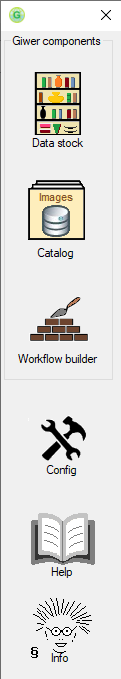
\includegraphics[height=13.5cm]{giwerMain.png}
	\caption{A Giwer keretrendszer}
	\label{fig:giwerStart}
\end{figure}

Itt indíthatjuk el a programok konfigurálását végző programrészt (\textit{Config} icon), valamint a program használatát segítő leírást, végül pedig a program metaadatait bemutató információs részt (\textit{About} ikon).

A \textit{DataStock} és a \textit{Workflow builder} önállóan is elindítható a keretrendszer nélkül, ha éppen úgy akarja a felhasználó.


\subsubsection{Data stock}

Ez az alkalmazás egy nagy, minolit program, amelyet interaktív működésre tervezünk. Számos függvényt fogunk implementálni, amelyek az adatok olvasását, írását, manipulálását végzik. Ezek a program menürendszerében fognak megjelenni, amit a felhasználó interaktívan, az egyes eljárások eredményességét vizsgálandó, aktivizálhat.

\begin{figure}[h]
	\centering
	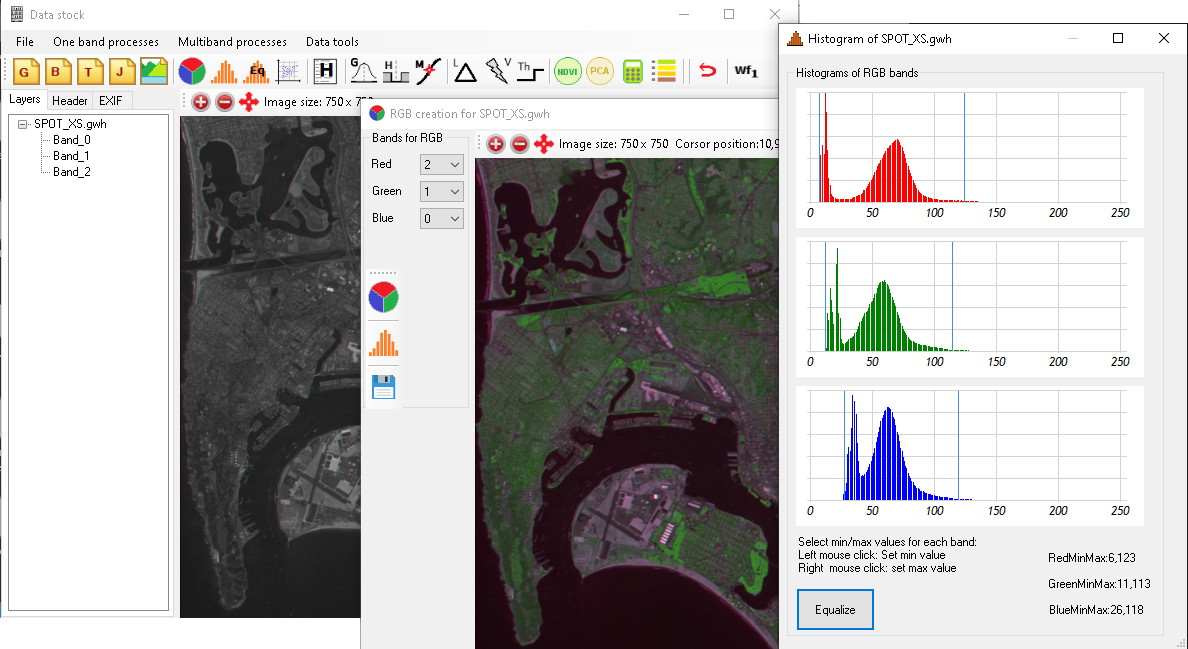
\includegraphics[width=14cm]{datastock1.png}
	\caption{A Data stock program egy képernyő képe}
	\label{fig:datastockStart}
\end{figure}

\subsubsection{Catalog}

A képek olyan nagy mennyiségben keletkeznek, hogy ezek áttekintése egy idő után reménytelen feladatnak látszik, és nagy a hibázás lehetősége. Ezért létrehozunk egy kép katalógust, egy nyilvántartó, kezelő alrendszert, amely adatbázisban tárolja, rendszerezi a képeket.

\subsubsection{Workflow builder}

A\textit{ Workflow builderrel} a rendelkezésre álló függvényekből tetszőleges munkafolyamatot (workflowt) állíthatunk elő.

\subsubsection{Config editor}

A \textit{Config} editorral, amelyet a keretprogramból indíthatunk el (\ref{fig:giwerStart}. ábra) a rendszer adatforrásait állíthatjuk be (\ref{fig:config}. ábra). Megadhatjuk, hogy hol találhatjuk a fájlrendszerben az idegen formátumú adatokat (\textit{bil}, \textit{tif}, \textit{jpg}), és a rendszer saját adatformátumú fájljait (\textit{gwh}).

\begin{figure}
\centering
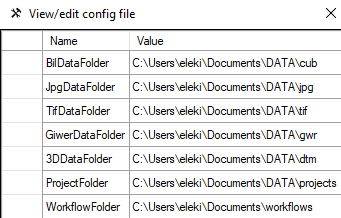
\includegraphics[width=4.5cm]{config.png}
\caption{A Config viewer/editor képernyő képe}
\label{fig:config}
\end{figure}

\subsubsection{Help}

A rendszer használatát angol nyelvű users' guide támogatja, amely a \textit{Help} ikonnal aktivizálható. Jelenleg ez még nem áll rendelkezésre. Várhatóan akkor fog elkészülni, amikor már alapvető változtatások nem várhatók a rendszerben.


\subsubsection{Getting information}

Az \textit{About} ikonra klikkeléssel a rendszer metaadatait nézhetjük meg (szerzők, verziószámok, copyright, stb.)

%*******************************************************************************************
\newpage
\part{Részletes leírás}

\setcounter{section}{0}

\section{A Giwer logikai felépítése}

Számos adatforrást kívánunk beolvasni (tif, jpg, bil, ddm) és vele műveleteket végezni. Az adatforrások közvetlen használata a feldolgozási műveletek során ugyan lehetséges, de nem elég gyors. Mivel gyakran óriási méretűek a képek, ezért a futási sebesség kritikus tényező, amit mindenképpen a lehető legkisebbre kell csökkenteni.

Ezért úgy gondoltuk, hogy saját adatformátumot fogunk használni, amely a gyors működést szolgálja. A nyers formátumoknak csak a megjelenítését biztosítjuk, hogy beolvasáskor lássuk, miről is van szó, de további műveletek nem engedélyezünk. Ha számításokat, képi elemzési funkciókat is szeretnénk végezni, akkor először át kell konvertáljuk a kívánt nyers fájlt \textit{gwr} formátumra (\ref{fig:gwr1}. ábra). A \textit{gwr} egy bináris formátum, amely egy frekvenciasáv intenzitás értékeit tartalmazza sorfolytonosan, ahol is egy pixel egy bájt. Ahány frekvenciasáv van a képben annyi bináris fájlunk lesz.

A számítási műveletek főként egy frekvenciasávon történnek, kivéve a többsávos műveleteket (pl. RGB kép generálás, főkomponens analízis, NDVI számítás, stb.). Gyakran a frekvenciasávonkénti műveletek eredményeit egyesítjük egy képben. 

Az eredmények megjelenítése igen lényeges része a funkcionalitásnak. A default megjelenítési stílus az, amikor greyscale-ként jelenik meg a kiválasztott frekvenciasáv. Számos számítási eredmény azonban éppen abban nyilvánul meg, hogy a kép intenzitás értékeit manipuláljuk, és a számított intenzitás értéknek fizikai jelentése van (pl. NDVI). Ezért szükséges, hogy olyan megjelenítést is alkalmazzunk, amely ezt a fizikai tartalmat teszi láthatóvá. Ilyenkor az RGB színmodellre alapuló 24 bites megjelenítés nem megfelelő. Ezért a megjelenítést nem 24 biten végezzük, hanem 8 bites color palette-t alkalmazunk, így a kép színes lesz, de legfeljebb 256 színű (\ref{fig:gwr1}. ábra). Ekkor lehetőség nyílik arra, hogy a számítási eredményekhez a legmegfelelőbb színeket alkalmazzuk (pl. hipszometrikus színes megjelenítés magassági adatokhoz, vagy osztályozott képeken az egyes osztályok eltérő színnel történő megjelenítése.)

\begin{figure}[h]
	\centering
	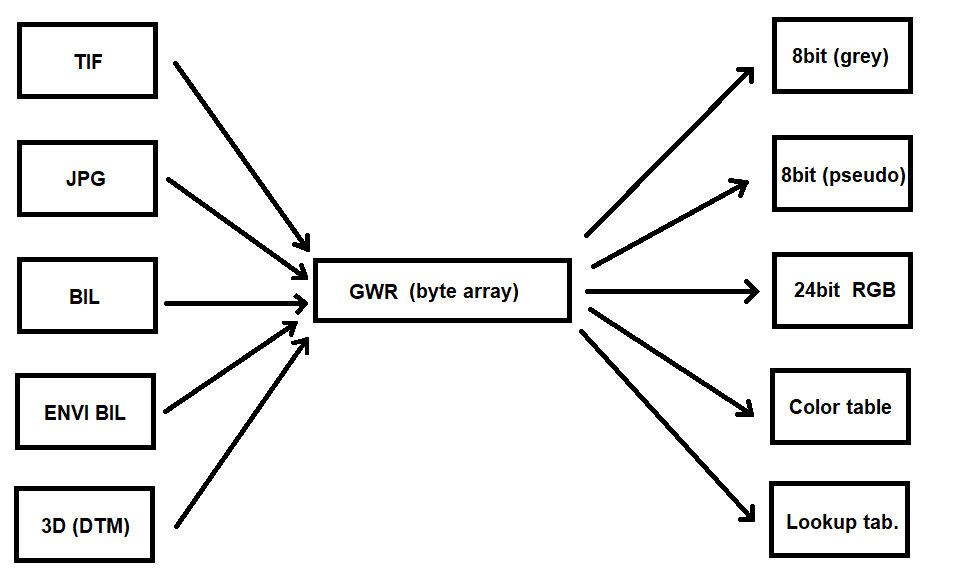
\includegraphics[width=10cm]{gwr1.png}
	\caption{A \textbf{Giwer} adatforrásai és konvertálása saját (gwr) formátumba. Valamennyi adatformátumot előbb gwr formátumba konvertáljuk, és csak azután végzünk velük számításokat. A megjelenítéshez, attól függően, hogy milyen típusú adatról van szó, és milyen színmodellt kíván a megjelenítés, vagy color táblás /8 bites/ vagy RGB /24 bites/ megjelenítést hajtunk végre.}
	\label{fig:gwr1}
\end{figure} 


\section{A Giwer keretrendszer}

A keretrendszer összefogja a különböző alkalmazásokat, segít konfigurálni a programot. Innen Indítható az interaktív desktop alkalmazás, a DataStock. Ugyancsak innen indítható a Workflow edit. Innen állíthatjuk be a program konfigurációs fájlját (config.cfg), amely a startup könyvtárban (ahol található az giwer.exe) található. Ez a fájl a forrásadatok (\textit{bil}, \textit{tif}, \textit{jpg}) elkérési útvonalát tartalmazza (DataFolder). A gwr formátumú adatok helyét is megadhatjuk itt (GiwerDataFolder). A Help segítségével megnyithatunk egy pdf fájlt, amely a program használatában segít. Az About röviden bemutatja a programot, és a különböző programkomponensek verziószámait.

\section{Data Stock}

A \textit{DataStock} raszteres képek beolvasását, manipulálását és az eredmények megjelenítését és tárolását végzi. Interaktív működésű. A rendelkezésre álló függvényeket a menürendszer által lehet meghívni. Számos képfeldolgozó eljárás lett beépítve, továbbá olyan adatkonverziós függvények, amelyekkel az optimális működéshez szükséges adatkonverziókat el lehet végezni.

\subsection{A program működése}

A \textit{DataStock} alrendszer tervezésekor saját adatformátum kidolgozását tartottuk a legcélszerűbbnek. Alapelv, hogy minden frekvenciasáv intenzitásértékeit egy-egy bináris fájlban tároljuk. A program ezeket az adatokat egy bytetömbben tartja, amivel gyorsan lehet műveleteket végezni. Mivel a képformátumok terén igen nagy a sokszínűség, ezért ezt a megoldást tartottuk a legjobbnak. Azáltal, hogy minden képet előbb saját formátumra hozunk (adat előkészítés), és az egységes adatszerkezeten végzünk műveleteket, így a későbbiekben könnyen bővíthetjük a támogatott fájlformátumok számát.

Kétféle műveletcsoportot hoztunk létre. Az egyik a \textit{OneBand functions} a másik a \textit{Multiband functions}. Az első csoportba azok a műveletek tartoznak, amelyek egyetlen frekvenciasáv adataival elvégezhetők (pl. digitális szűrések egy frekvenciasávra, hisztogram kiegyenlítés, adatkonverziók, stb.) A másik csoportba azok a funkciók tartoznak, amelyek egyszerre több frekvenciasáv adatait igénylik (pl. RGB képek létrehozása, PCA, NDVI, stb.)

A főbb funkciókörök a következők:

\begin{itemize}
	\item különböző adatformátumú képek beolvasása és konverziója (\textit{tif}, \textit{jpg}, \textit{bil}, \textit{gwh})
	\item képek megjelenítése
	\item egy és többsávos képfeldolgozási műveletek végrehajtása, amelyek a későbbiekben részletesen is be lesznek mutatva
\end{itemize}

\subsection{Támogatott adatformátumok}

Háromféle raszteres adatformátum beolvasását támogatja a program: \textit{bil}, \textit{tif} és \textit{gwr} (a \textit{Giwer} saját bináris adatformátuma). 

\subsubsection{Tiff}
A \textit{tif} a jól ismert tagged image format, amelynek egy speciális, térinformatika célú változatát, a geo tiffet is használjuk. Ez a formátum nemcsak pixelenkénti intenzitás értékeket tárol, hanem a headerben a kép georeferencia adatait (vetületi rendszer, kalibrációs pontok /többnyire sarok pont koordináták/ egyéb a képalkotásra vonatkozó adatok). Részletes leírása megtalálható a következő linken: 

\noindent
\textit{https://earthdata.nasa.gov/esdis/eso/standards-and-references/geotiff}

Hagyományos \textit{tiff} formátumot is támogat a program, amely nem tartalmaz georeferencia adatokat. Ilyenkor máshonnan vesszük a képek térbeli referencia adatait. Általában minden tif kép tartalmaz \textit{exif} adatokat, amelyek olvashatók. Mivel az \textit{exif} nem szabvályos, így az olvasásával számos nehézség előfordul. Például DJI drónra szerelt multispektrális Micasense és az RGB Zenmuse kamerák minden repülési adata, mint pl. drón pozíció, kép orientáció (északi iránnyal bezárt szög), képméret, sávok száma, színmélység, stb. az exif-ben van tárolva. Ezeket csak erre a célra kidolgozott eljárásokkal tudjuk olvasni.


\subsubsection{Jpeg}

A jól ismert \textit{jpg} formátumú képek beolvasását is támogatja a program. Ez többnyire nem tartalmat georeferencia adatokat. Bizonyos esetekben léteznek hozzá kiegészítő fájlok, amelyek tartalmaznak a vetületi rendszerre, kalibrációs pontokra vonatkozó adatokat. Drón képek esetén ilyen fájlok nincsenek, csak a hagyományos \textit{jpg} fájl. Hasonlóan a tiff fájlokhoz, a jpg fájlok leíró adatait, a replüléssel összefüggő kép adatokat csak erre a célra kidolgozott \textit{exif} eljárásokkal lehet beolvasni.

\subsubsection{Bil}
A \textit{bil} egy speciális formátum, amelyet soksávos űrfelvételek tárolására dolgoztak ki. Részletes leírása megtalálható a következő linken:

\noindent
\textit{http://desktop.arcgis.com/en/arcmap/10.3/manage-data/raster-and-images/bil-bip-and-bsq-raster-files.htm}

\begin{figure}
	\centering
	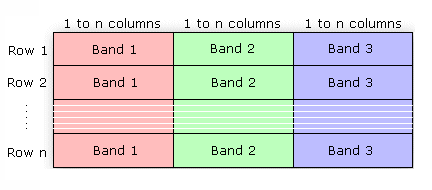
\includegraphics[width=11cm]{bil_struc1.png}
	\caption{A \textit{BIL} fájl adatstruktúrája}
	\label{fig:bilstruc1}
\end{figure}

Röviden összefoglalom a \textit{BIL} leírását, mert kiemelt jelentőségű, és a harmadik formátum, \textit{gwr} ismertetéséhez is szükség lesz rá. A \textit{BIL} a Band Interleaved by Line szavak rövidése, amelyet multispektrális (vagyis több frekvenciasávos) képek tárolására fejlesztettek ki. A \textit{BIL} önmagában nem képformátum, hanem a kép tényleges pixelértékeinek fájlban való tárolására szolgáló adatstruktúra. A \textit{BIL} támogatja az egy- és többsávos képek tárolását legyen az fekete-fehér, a szürkeárnyalatos, a pszeudo color, true color vagy multispektrális esetleg hiperspektrális.



A \textit{BIL} fájlhoz, amely bináris, tartozik egy header fájl is (ASCII fájl), amely alapján a \textit{BIL}-ben található bináris adatok értelmezhetők. Kiegészítő adatokat tartalmaz a képről, mint például a képen látható sorok és oszlopok számát, a frekvenciasávok száma, színmélység (bits per pixel), sarokpont adatok földi koordináta rendszerben, bájt sorrend, egy pixel mekkora valós terület reprezentál, stb.

\begin{figure}
	\centering
	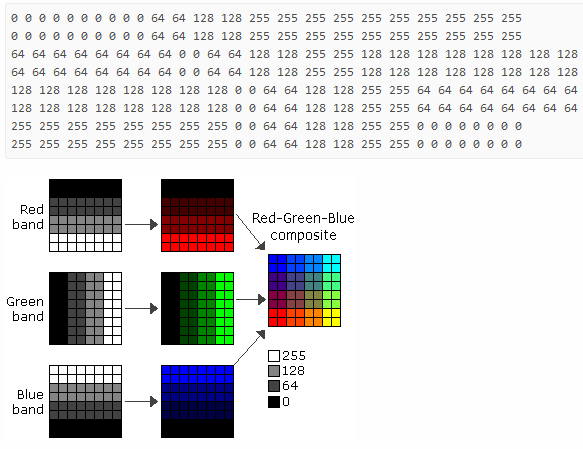
\includegraphics[width=14cm]{bil_struc2.png}
	\caption{Egy képi példa \textit{BIL} fájl adatstruktúrájára}
	\label{fig:bilstruc2}
\end{figure}

A \textit{BIL} sávonként tárolja a kép minden sorát. Például, ha egy háromsávos képünk van, akkor az 1. sor mindhárom sávját tároljuk az 1. sorban, majd a 2. sor  mindhárom sávját, és így tovább, amíg el nem érjük a képen a sorok számát. A \ref{fig:bilstruc1}. ábra egy három sávos \textit{bil} fájl adatait szemlélteti. Ha az ábrát sorfolytonosan nézzük, akkor megkapjuk a disken lévő \textit{bil} hosszú sorvektorát. 



\subsubsection{DDM}

A \textit{DDM} formátum a magyar digitális domborzatmodell bináris adatformátuma, amely sorfolytonosan tárolja a pontonkénti magasság adatokat. Egy magasságadat 2 byte. Az bináris adatok metaadatait egy header fájl tartalmazza textként, amelyből kiolvashatók az adatsor főbb paraméterei, mint pl. a sorok és oszlopok száma, a pixel fizikai mérete, a sarokpont koordináták, a koordináta rendszer, és még néhány apróság. A \ref{fig:ddm1}. ábrán a Dunakanyar digitális terepmodelljét láthatjuk.

\begin{figure}
	\centering
	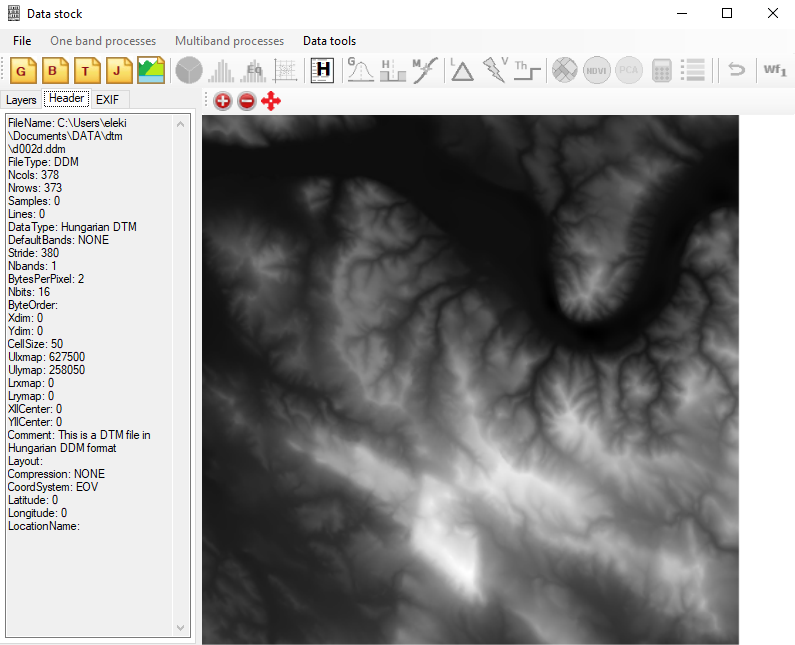
\includegraphics[width=14cm]{ddm1.png}
	\caption{A Dunakanyar digitális terepmodellje grayscale képként ábrázolva. A legalacsonyabb értékek feketével, a legmagasabbak fehérrel vannak jelölve}
	\label{fig:ddm1}
\end{figure}

\subsubsection{Gwr}

A \textit{gwr} egy bináris fájlformátum, amely a frekvenciasávok pixelértékeit egy-egy különálló fájlban tárolja. Ehhez is tartozik egy header fájl (\textit{gwh}), amely metaadatokat tartalmaz a képről, hasonlóan a \textit{bil} headeréhez.



\subsection{Osztályok és függvények}

A következőkben bemutatjuk, hogy mely osztályok, és mely függvények teszik lehetővé a fentebb vázlatosan bemutatott funkcionalitást:

\subsubsection{A \textbf{GeoImageData} osztály}

A \textbf{GeoImageData} osztály a képek header fájljainak beolvasására és parszolására hivatott. A fájlnév megadása révén a \textbf{GeoImageData} osztály tulajdonságai felveszik azt az értéket, amelyeket a fájlból kiolvasott. Az osztály főbb függvényei láthatók a \ref{fig:GeoImageData}. táblázatban.


\begin{table}
\begin{small}	
\begin{tabular}{|l|l|l|l|}
	\hline
	\textbf{Name} & \textbf{Function} & \textbf{DataIn} & \textbf{DataOut}\\	
	\hline
	parseGiwerHeader & read Giwer header & File name (string) & properties \\
		\hline
	parseBilHeader & read Bil header & File name (string) & properties \\
		\hline
	parseTifHeader & read Tif & File name (string) & properties \\
		\hline
	parseJpgHeader & read jpg & File name (string) & properties \\
		\hline
	parseTifParams & read Tif & File name (string) & properties \\
		\hline
	parseGeoTifParams & read geoTif & File name (string) & properties \\
		\hline
	get Exif data& read Exif & File name (string) & properties \\
		\hline
	compute Bil stride & compute stride &  & properties \\
	\hline
\end{tabular}
\end{small}
	\caption{A \textbf{GeoImageData} osztály főbb függvényei}
	\label{fig:GeoImageData}
\end{table}


\subsubsection{A \textbf{GeoImageTools} osztály}

A \textbf{GeoImageTools} számos eljárást tartalmat, amelyek a képek előfeldolgozásához, különféle konverziókhoz, manipulációkhoz szükségesek. Vázlatos leírásuk a \ref{fig:GeoImageTools}. táblázatban láthatók.

\begin{table}
	\begin{small}	
		\begin{tabular}{|l|l|l|l|}
			\hline
			\textbf{Name} & \textbf{Function} & \textbf{DataIn} & \textbf{DataOut}\\	
			\hline
			readGwrFile & read source data file & File name & byte[ ] \\
				\hline
			convertOneBandBytes & convert image from a  & byte[ ] & bitmap \\
			toBitmap & given band into bitmap & &\\
				\hline
			byteArray2Bitmap & convert bytearray to& byte[ ] & bitmap \\
			&a bitmap & &\\
				\hline
			bitmap2ByteArray & convert bitmap & bitmap & byte[ ] \\
			&  to a bytearray & &\\
				\hline
			getAnRGBBand& get a band data  & which band & byte[ ] \\
			& from a bytearray & &\\
				\hline
			getOneBand2Bytes & get a band data & which band & byte[ ] \\
			& from a bytearray &&\\
				\hline
			combine2Images & combine current  & byte1[ ], byte2[ ] & byte[ ] \\
			&image with another& &\\
				\hline
			vectorize & vectorize an image & byte[ ], params & byte[ ] \\
				\hline
			thresholding & thresholding & byte[ ], params & byte[ ] \\
				\hline
			computeHistogram & compute histogram  & byte[ ] & float[ ] \\
			& of a bytearray & &\\
				\hline
			HistoEqualization & histogram equalization & byte[ ] & byte[ ] \\
				\hline
			grayscale & grayscale conversion & byte[ ] & byte[ ] \\
				\hline
			invertColor & color inversion & byte[ ] & byte[ ] \\
				\hline
			convert2GiwerFormat & convert images (tif,jpg,bil)  & File name & byte\\	
			&to Giwer format & &\\
				\hline
			saveGiwerFormat & save a bytearray  & File name  & File name\\	
			&to gwr file format & &\\
				\hline
			convertImagefromTif2Jpg & convert an image & bitmap&bitmap\\
			& from tif to jpg & &\\
				\hline
			convertImagefromJpg2Tif & convert an image & bitmap&bitmap\\
			& from jpg to tif & &\\	
			\hline
		\end{tabular}
	\end{small}
	\caption{A \textbf{GeoImageTools} osztály függvényei}
	\label{fig:GeoImageTools}
\end{table}

\subsubsection{A \textbf{StatMath} osztály}

A \textbf{StatMath} osztály matematikai eljárásokat tartalmaz, amelyek szerepet kapnak a képfeldolgozás során. Ezekt láthatjuk a \ref{fig:StatMath}. táblázatban.

\begin{table}
	\begin{small}	
		\begin{tabular}{|l|l|l|l|}
			\hline
			\textbf{Name} & \textbf{Function} & \textbf{DataIn} & \textbf{DataOut}\\	
			\hline
			getMinMax&compute image & int[] or double[]&string\\
			&min, max values&&\\
			\hline
			imageAverage & compute image's mean& byte[ ]&float\\	
			\hline
			imageScatter & compute image's scatter& byte[ ]&float\\	
			\hline
			imageStandardization & compute standardized& byte[ ],  &byte[ ]\\	
			& image&double, double&\\
			\hline			
			compCorrelationMatrix&compute corr.matrix& list of bands& byte[ ]\\
			\hline
			compEigen & compute eigenvectors & byte[ ]&Eigenvalues\\
			&and eigenvalues & & and vectors\\
			\hline
			PCA & compute the desired& N * byte[ ], &byte[ ]\\
			&  principal component & eigens&\\

			\hline
		\end{tabular}
	\end{small}
	\caption{A \textbf{StatMath} osztály főbb függvényei}
	\label{fig:StatMath}
\end{table}


\subsubsection{A \textbf{GeoFilters} osztály}

A \textbf{GeoFilters} osztály különböző digitális szűrések függvényeit tartalmazza. A lista még távolról sem teljes. Egyelőre csak azok vannak benne, amelyek már működnek. Valamennyi függvény egyetlen, általunk kiválasztott frekvenciasávra működik, kivéve, amelyek kifejezetten RGB sávokra működnek. Vázlatos leírásuk a a \ref{fig:GeoFilters}. táblázatban láthatók.


\begin{table}
	\begin{small}	
		\begin{tabular}{|l|l|l|l|}
			\hline
			\textbf{Name} & \textbf{Function} & \textbf{DataIn} & \textbf{DataOut}\\	
			\hline
			medianFilter1Band & median filtering & byte[ ], kernel & byte[ ] \\
			& on one band&&\\
			\hline		
			medianFilte3Band & median filtering & byte1[],byte2[],byte3[], & byte[ ] \\
			&  on 3 bands&  kernel&\\
			\hline
			LaplaceOneBand & Laplace filtering & byte[ ] & byte[ ] \\
			&on one band&&\\
			\hline
			Laplace3Bands & Laplace filtering & byte1[ ],byte2[],byte3[] & byte[ ] \\
			&on 3 bands&&\\
			\hline
			convolSingleBand& convolution filtering & byte[ ] & byte[ ] \\
			&on one band&&\\
			\hline
			convol3Bands & convolution filtering & byte1[],byte2[],byte3[] & byte[ ] \\
			&on 3 bands&&\\
			\hline
			highPassKernel & Laplace filtering & float & double[,] \\
			&on one band&&\\
			\hline
			lowPassKernel & Laplace filtering & float & double[,] \\
			&on 3 bands&&\\
			\hline
			lowPassKernelGauss& convolution filtering & float & double[,] \\
			&on one band&&\\
			\hline
			resampling & convolution filtering & int rate, bitmap & byte[ ] \\
			&on 3 bands&&\\
			\hline
			gradientFilter & convolution filtering &byte[ ]  & byte[ ] \\
			&on 3 bands&&\\
			\hline
		\end{tabular}
	\end{small}
	\caption{A \textbf{GeoFilters} osztály főbb függvényei}
	\label{fig:GeoFilters}
\end{table}

\subsubsection{A \textbf{GeoMultibandMethods} osztály}

A \textbf{GeoMultibandMethods} osztály olyan függvényeket tartalmaz, amelyek egynél több frekvenciasávra működnek.  Vázlatos leírásuk a \ref{fig:MultibandMethods}. táblázatban láthatók. 


\begin{table}
	\begin{small}	
		\begin{tabular}{|l|l|l|l|}
			\hline
			\textbf{Name} & \textbf{Function} & \textbf{DataIn} & \textbf{DataOut}\\	
			\hline
			NDVI & computes NDVI & byte1[], byte2[] & byte[] \\
			\hline
			clustering & clustering & N * byte[ ] or PC1 & byte[] \\
			\hline
			Segment & segmentation & N * byte[ ] or PC1 & byte[] \\
			\hline
			createRGB\_gwr & creates an RGB image & byte1[],byte2[],byte3[]& bitmap \\
			& from 3 bytearrays&&\\
			\hline
			crossPlot& create cross-plot& byte1[], byte2[] & byte[] \\
			& from 2 bands &&\\
			\hline
		\end{tabular}
	\end{small}
	\caption{A \textbf{GeoMultibandMethods} osztály főbb függvényei}
	\label{fig:MultibandMethods}
\end{table}

\subsubsection{A \textbf{DTM} osztály}

A DTM osztály digitális domborzati modellek (digital terrain modell) kezelését szolgálja. Segítségével raszteres adatszerkezetű magassági adatok olvashatók be, és jeleníthetők meg. Egyelőre több funkciót nem valósítottunk meg, de az adatok a Giwer saját formátumában rendelkezésre állnak további feldolgozó függvények számára.

\subsubsection{A \textbf{Raster calculator} osztály}

A raszter kalkulátor arra szolgál, hogy segítségével megadott feltételek szerint lekérdezést hajthassunk végre az aktuális képre. Ez egyrészt azt jelenti, hogy kiemelhetünk a képből olyan területeket, amelyet hangsúlyosabban kívánunk láttatni, másrészt a legyűjtés eredményeként létrejött képen tetszőleges további műveleteket hajthatunk végre.

\subsubsection{Az \textbf{ImageWindow} osztály}

Az \textbf{ImageWindow} osztály képek megjelenítésére szolgál. Nemcsak a bemenő képek szemlélhetünk általa, hanem bármely művelet eredményét is megnézhetjük. Vázlatos leírása a \ref{fig:ImageWindow}. táblázatban látható.


\begin{table}
	\begin{small}	
		\begin{tabular}{|l|l|l|l|}
			\hline
			\textbf{Name} & \textbf{Function} & \textbf{DataIn} & \textbf{DataOut}\\	
			\hline
			loadImageFromFile & load an image from  & file & Load and display \\
			&a file && image\\
			\hline
			clear & clear screen &  & empty screen \\
			\hline
			zoomIn & image zoom in & byte[] & zoomed image \\
			\hline
			zoomOut&image zoom out & byte[] & zoomed image \\
			\hline
			DrawImage & draw an image from & byte[]  &  \\
			&a byte array&&\\
			\hline
			DrawImageRGB & draw an image from & byteR[],byteG[], &  \\
			&RGB byte arrays&byteB[] &\\
			\hline
			DrawImageDDM & draw elevation data& byte[], float[,]  &  \\
			&from a byte array&&\\
			\hline			
		\end{tabular}
	\end{small}
	\caption{A \textbf{ImageWindow} osztály főbb függvényei}
	\label{fig:ImageWindow}
\end{table}

A fenti függvények biztosítják a képek zoomolását, de annak sokkal többet is tud az \textbf{ImageWindows} osztály. A betöltött kép fölött mozgatott kurzor pozícióját is megjeleníti, sőt a kép adott pozíciójának értékét is megmutatja. Ez többnyire egy 24 bites RGB érték, egy 8 bites grayscale kép, de lehet egy csoportba tartozási érték is. Ebben az esetben a kép megjelenését a lookup table határozza meg, amely meghatározza, hogy a 8 bites kép milyen színtábla (colortable) szerint jelenik meg.

Ha domborzati adatokat tartalmaz a kép, akkor a kurzos pozícióján kívül, az ehhez a pozícióhoz tartozó magasságértékeket is megmutatja. Ha a lookup table nem \textit{default}ra van állítva (greyscale), hanem \textit{hipsometric}-re, akkor a 8 bites képet színesben fogjuk látni, ahol a színek a különböző magasságokat szimbolizálják.


\subsection{A \textbf{Project} osztály}

A drónok általában nagy tömegben hoznak létre képeket, emiatt célszerű őket projektbe szervezve feldolgozni. Olyankor is hasznos lehet a projekt használata, ha egyszerre több képpel foglalkozunk. Ilyenkor a projekt nevével hivatkozhatunk arra a gyűjteményre, amelybe összegyűjtöttük a használni kívánt képeket.

\subsection{A \textbf{Mosaic} osztály}

Amikor sok drón kép készül egy adott területről, akkor ezek a képek valamekkora átfedéssel (általában 50-75 \%-os átfedés) képezik le a kívánt terület. Ezek megjelenítése különösen problematikus. Nem járható az az út, hogy egyetlen hatalmas képpé ragasszuk össze a képeket, ezért meg kell maradjanak a képek önállónak, de egyszerre kell tudni megjeleníteni őket, sőt a feldolgozási folyamatokat is egyszerre kell futtassuk. 



\section{Függvények és eljárások bemutatása}

Ebben a részben röviden bemutatjuk a \textbf{Giwer} rendszerbe beépített eljárások és függvények működését, elvi hátterét.

\subsection{A \textbf{GeoImageData} osztály eljárásai}

Ez az osztály arra hivatott, hogy támogatott képformátumok metaadatait beolvassa és tárolja. Egységesen, minden képhez ugyanazokat a property-ket, ugyanolyan néven  hozza létre, függetlenül attól, hogy eredetileg milyen név volt a forrás header fájlban. A következő eljárásai vannak: parseGiwerHeader, parseTifHeader, parseBilHeader, parseJpgHeader, parseExif. Ennek jelentősége abban van, hogy ha később bővülne a támogatott fájl formátumok száma (pl. ENVI headert is kezelni szeretnénk), akkor emiatt nem kell módosítanunk a többi osztály működésén, mert minden művelet a \textbf{GeoImageData} osztályt használja.


\subsubsection{parseBilHeader}

Ez a függvény beolvassa, és betölti a \textit{bil} fájl headerjének tartalmát a \textbf{GeoImageData} osztály propertyjeibe. Mivel sokféle bil fájl létezik, ezért nem minden property kap értéket, de valamennyi kiszámítható valamely másikból. Ezeket a számításokat a Giwer elvégzi.

\subsubsection{parseTifHeader}

Ez a függvény beolvassa a \textit{tif} fájl metaadatait, és betölti a \textbf{GeoImageData} osztály propertyjeibe. Külön függvény végzi a \textit{geotif} formátumú képek paramétereinek beolvasását (parseGeoTifParams), amelyhez az open source gdal library-t is felhasználtuk. A drónok által szolgáltatott képek nem georeferált fotrmátumkat használnak, ezért ezeket külön erre a célra kifejlesztett eljárással olvassuk be (parseTifParams és parseJpgParams).


\subsubsection{parseGeoTifHeader}

Mivel a hagyományos \textit{Tif} fájl nem tartalmaz georeferencia adatokat, ezért szükséges a GeoTif formátumra külön parsolót készíteni. Noha a pixelek olvasása hasonlóan történhet, mint a hagyományos Tif fájlok esetében, de a fájl headerben további beolvasandó adatok vannak (pl. Datum, szferoid adatok, vetületi rendszer, a vetületi egyenletek paraméterei, stb.), amelyeknek az ismerete szükséges további feldolgozások számára. Ez a függvény ezeket az adatok beölti  a \textbf{GeoImageData} osztály propertyjeibe.

\subsubsection{parseJpgHeader}

Ez a függvény beolvassa a \textit{jpg} fájl metaadatait, és betölti a \textbf{GeoImageData} osztály propertyjeibe. Nem minden property kap értéket, hiszen például a drónok által alkotott képek nem georeferáltak, így koordináta információt nem tartalmaznak. Ezeket más módon kell megállapítani, és betölteni a \textbf{GeoImageData} osztály propertyjeibe.

\subsubsection{getExif}

Ez a függvény a \textit{tif} és \textit{jpg} formátumú fájlok exif adatait olvassa be. Ezek között szerepelhetnek georeferencia adatok is, ha \textit{geotif} vagy \textit{geojpg} a fájlok formátuma. Ezenkívül az exponálással kapcsolatos adatok is (expozíciós idő, blende nyílás, kamera típus, stb.) szerepel az adatok között.


\subsubsection{parseGiwerHeader}

Ez a függvény a \textit{gwh} formátumú header fájl adatait olvassa be, és tölti be a \textbf{GeoImageData} osztály propertyjeibe. Ez a fájl csak akkor létezik, ha előzőleg valamely más formátumú adatot (\textit{bil}, \textit{tif}, \textit{jpg}) már átkonvertáltunk \textit{gwr} formátumba.




\subsection{A \textbf{GeoImageTools} osztály eljárásai}

Ebben a fejezetben áttekintjük a \textbf{GeoImageTools} osztály eljárásait.

\subsubsection{saveGiwerFormat}

Ez a függvény elmenti valamely forrásfájl képét \textit{gwr} formátumban. Megadható a mentendő fájl neve, és helye. A megadott néven létrehoz egy header fájlt (gwh), amely a kép metaadatait tartalmazza, valamint egy a kiterjesztés nélküli fájl néven egy könyvtárat, ahová a bináris adatok bekerülnek 0,1,2 ...   fájlnéven, annyiadik számon, ahányadik csatorna képét tartalmazza.

\subsubsection{saveHeader2Giwer}

Ez a függvény a a metaadatokat giwer header (gwh) formátumban menti el.

\subsubsection{convertByteArray2GiwerFormat}

Ez a függvény az adott byte tömb tartalmát menti el giwer formátumban, a megadott helyen és néven.

\subsubsection{convertOneBandBytestoBitmap}

Ez a függvény egy byte tömb adataiból egy bitmapet készít. Mivel egyetlen sávról van szó, a bitmap egy szürke kép lesz, mivel a bitmap mindhárom színcsatornájában ugyanannak a byte tömbnek az adatai vannak.

\subsubsection{getOneBandBytes}

Ez a függvény kiolvassa egy csatorna byte adatait és egy byte tömbbe tölti.

\subsubsection{getOneBandtoByteArrayFromBitmap}

Ez a függvény egy bitmapből kiolvassa a megadott színsáv adatait és egy byte tömbbe tölti.

\subsubsection{BitmapToByteArray}

Ez a függvény egy adott bitmapet három színsávra bont, és ezeket egy-egy byte tömbbe tölti.

\subsubsection{ByteArrayToBitmap}

Ez a függvény egy vagy három byte tömbben tárolt kép adataiból egy bitmapet számol.

\subsubsection{convertImageFromTif2Jpg}

Ez a függvény tif-ből jpg-be konvertálja a megadott fájlt.

\subsubsection{convertImageFromJpg2Tif}

Ez a függvény jpg-ből tif-be konvertálja a megadott fájlt.

\subsubsection{InvertColor}

Ez a függvény invertálja at adott bitmap képét

\subsubsection{GrayscaleConversion}

Ez a függvény egy bitmapet szürkévé alakít.

\subsubsection{readGwrFile}

Ez a függvény beolvas egy giwer formátumú fájlt.



\subsubsection{GetAnRGBBand}

A képek feldolgozása szempontjából nem alapvető jelentőségű, de vizualizációs szempontból hasznos lehet, ha meg tudjuk mutatni egy-egy kép RGB színsávjait az alapszínekben ábrázolva. Erre szolgál a getAnRGBBand(WhichBand) függvény, ahol meg kell adnunk, hogy mely RGB sávot szeretnénk látni (whichBand). Eredménye egy bitmap, amelyet megmutat az ImageWindow (\ref{fig:redBand}. ábra). További számítások az eredménnyel nem végezhetők.

\begin{figure}
	\centering
	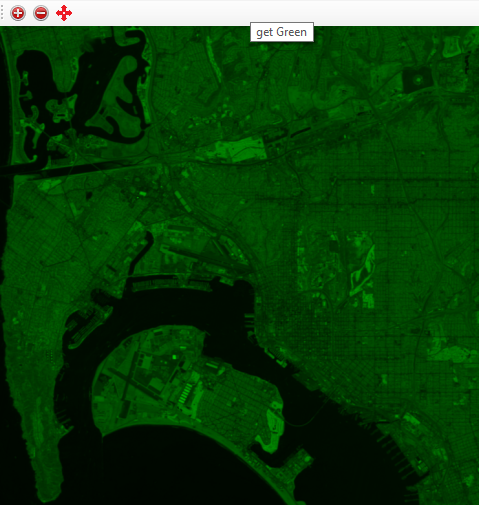
\includegraphics[width=12cm]{redBand.png}
	\caption{A zöld sáv megmutatása}
	\label{fig:redBand}
\end{figure}

\subsubsection{combine2Images}

Ez függvény az aktuális képet kombinálja egy tetszőleges másikkal. Egyelőre három művelet készült el: az összeadás, a kivonás és a kizáró vagy (EXOR) művelet. A '+' és a '-' művelet funkciója nyilvánvaló. Az 'exor'-t olyankor használjuk, amikor az egyik képet úgy kombináljuk egymással, hogy bizonyos feltételek teljesülése esetén vagy csak az egyik vagy csak másik legyen a kombinált kép tartalma (\ref{fig:datastock_cloud1}. ábra).

\begin{figure}
\centering
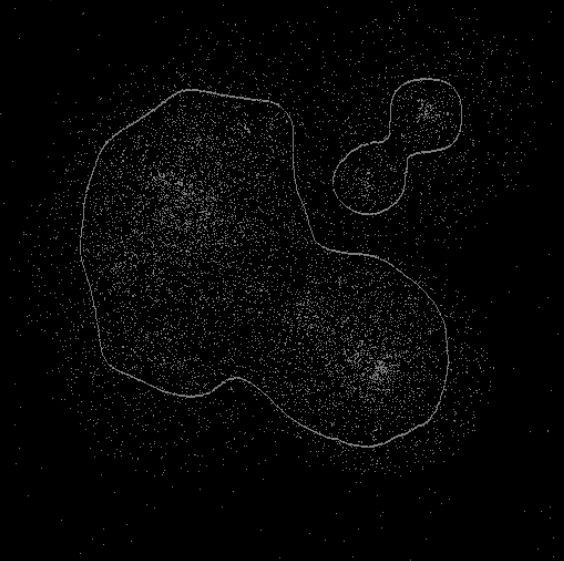
\includegraphics[width=10cm]{datastock_cloud1.png}
\caption{Két kép kombinációja \textit{EXOR} művelettel. Az egyik kép egy RGB image a pontfelhőről, a másik pedig a pontfelhő határait mutatja}
\label{fig:datastock_cloud1}
\end{figure}

\subsection{A \textbf{StatMath} osztály eljárásai}

\subsubsection{getMinMax}

Ez a függvény kiszámítja egy byte tömbben tárolt kép minimális és maximális intenzitásértékét.

\subsubsection{imageAverage}

Ez a függvény kiszámítja egy byte tömbben tárolt frekvenciasáv intenzitásértékeinek átlagát.

\subsubsection{imageScatter}

Ez a függvény kiszámítja egy byte tömbben tárolt frekvenciasáv intenzitásértékeinek szórását.

\subsubsection{imagesStandardization}

Ez a függvény standardizál egy byte tömbben tárolt képet

\subsubsection{computeCorrelationMatrix}

Ez a függvény kiszámítja tetszőleges számú, byte tömbben tárolt képek korrelációs mátrixát

\subsubsection{compEigen}

Ez a függvény kiszámítja egy mátrix sajátértékeit és sajátvektorait

\subsubsection{PCA}

Ez a függvény kiszámítja tetszőleges számú, byte tömbben tárolt kép bármely főkomponensét



\subsection{A \textbf{GeoFilters} osztály eljárásai}

A \textbf{GeoFilters} osztály olyan eljárásokat tartalmaz, amelyek egy kiválasztott frekvenciasávra vonatkozó szűréseket végeznek.

\subsubsection{MedianFilter3Bands}

Ez a függvény mediánszűrést végez három megadott frekvenciasáv intenzitásértékeit tartalmaz byte tömbökre. A kernel hosszát bemenő paraméterként kell megadni.

\subsubsection{MedianFilterOneBand}

Ez a függvény mediánszűrést végez egy megadott frekvenciasáv intenzitásértékeit tartalmazó byte tömbre. A kernel hosszát bemenő paraméterként kell megadni.


	
\subsubsection{Canny}

Ez a függvény éldetektálást végez egy megadott frekvenciasáv intenzitásértékeit tartalmaz byte tömbre a Canny-féle eljárás alapján.

\subsubsection{Laplace3Bands}

Ez a függvény éldetektálást végez három megadott frekvenciasáv intenzitásértékeit tartalmazó byte tömbökre a Laplace-féle eljárás alapján.

\subsubsection{LaplaceOneBand}

Ez a függvény éldetektálást végez egy megadott frekvenciasáv intenzitásértékeit tartalmazó byte tömbre a Laplace-féle eljárás alapján (\ref{fig:laplace1}. ábra).

\begin{figure}
	\centering
	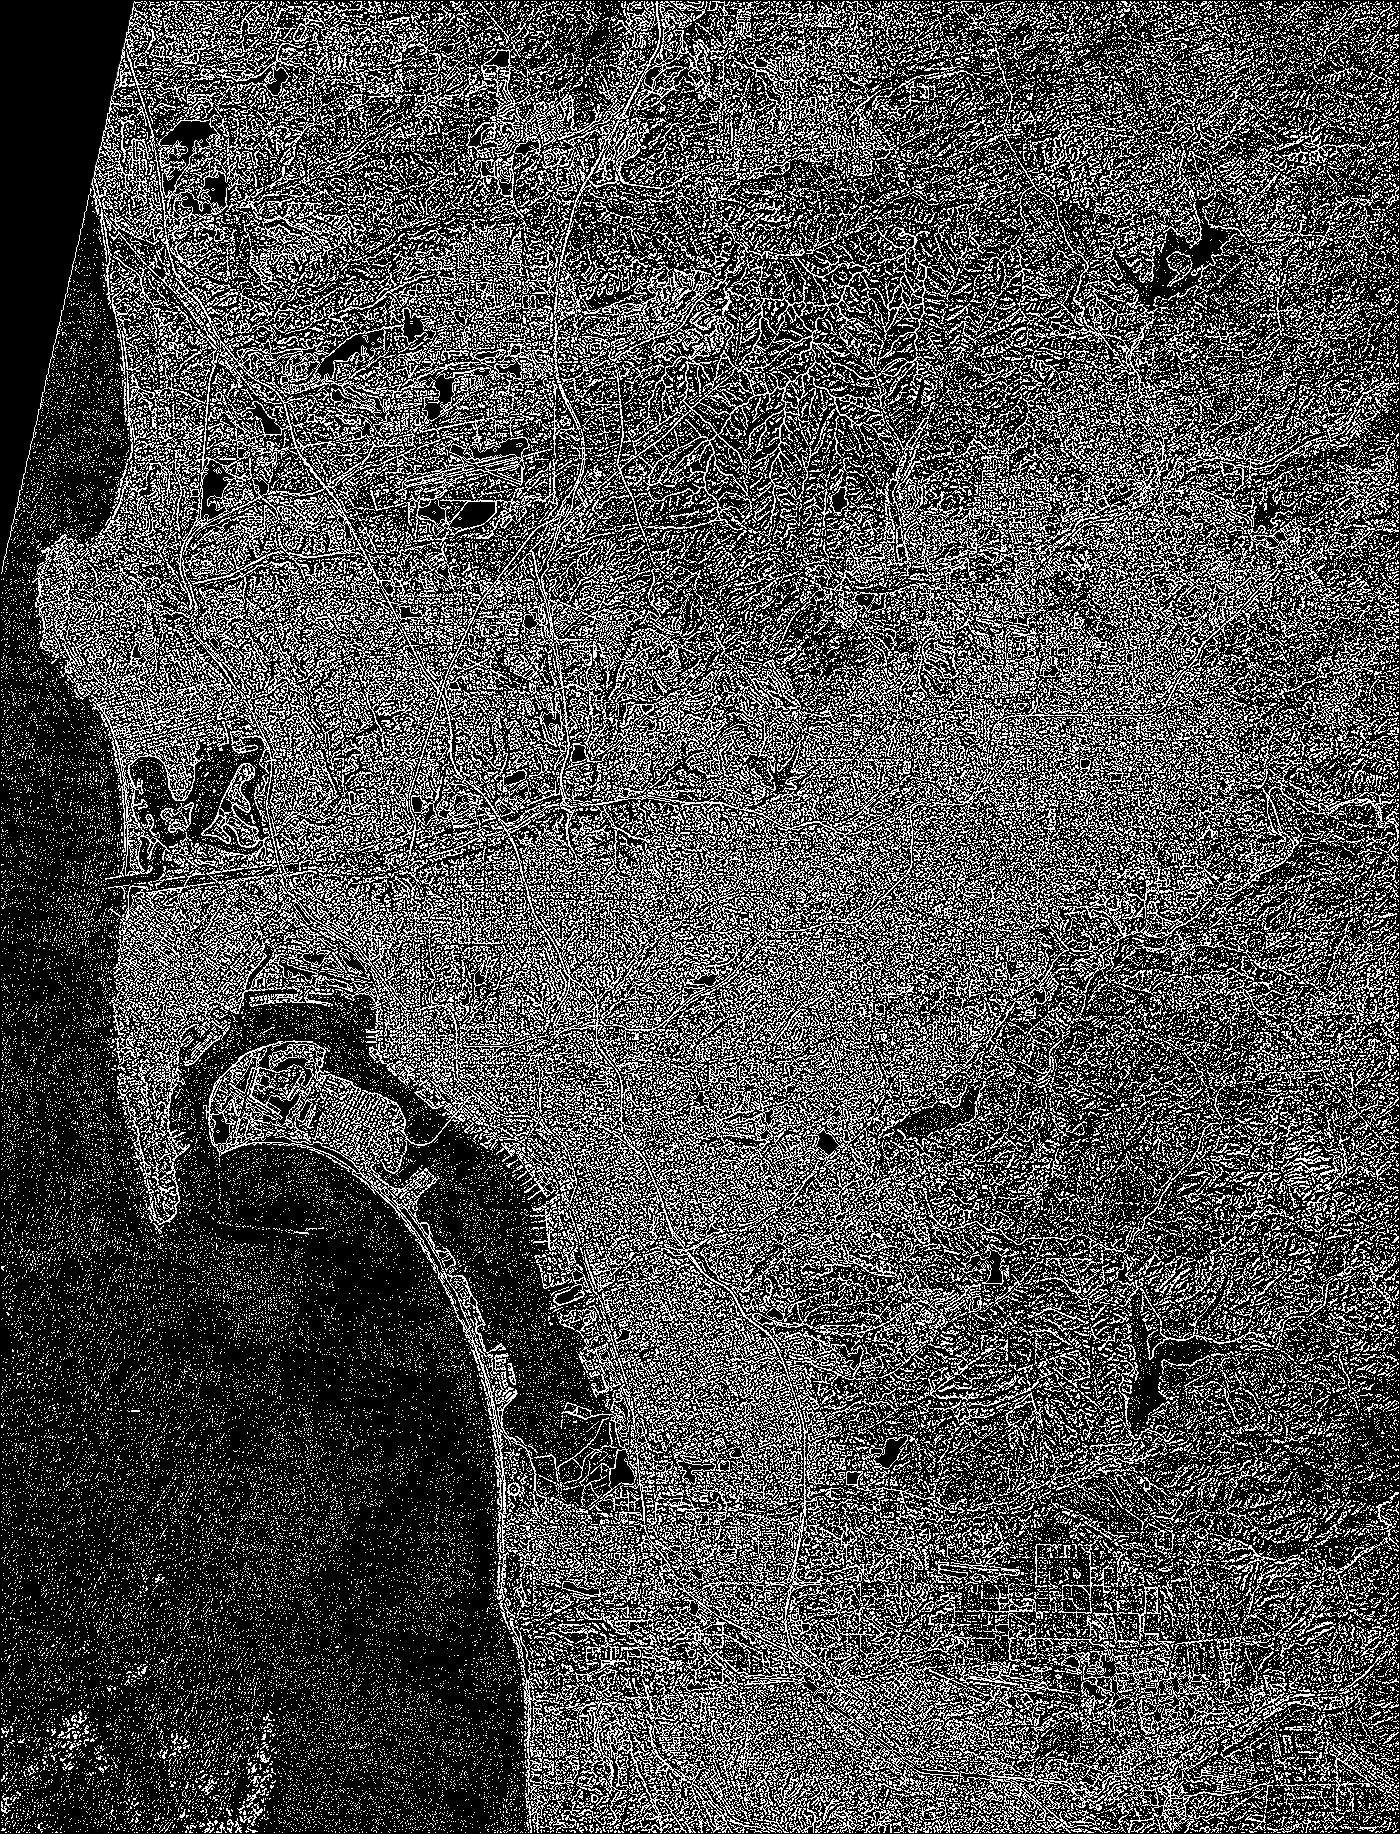
\includegraphics[width=12cm]{laplace1.png}
	\caption{A Laplace-szűrés eredménye az egyik frekvenciasávra}
	\label{fig:laplace1}
\end{figure}

Itt kell megjegyezni, hogy mivel a Laplace-szűrés egy második deriválton alapuló szűrő, ezért érzékeny a zajokra, így érdemes előtte valamilyen simító szűrést alkalmazni (Gauss-simítás vagy medián szűrő), és csak azután végezni el a Laplace szűrést. Ennek eredményét mutatja a \ref{fig:laplace2}. ábra.

\begin{figure}
	\centering
	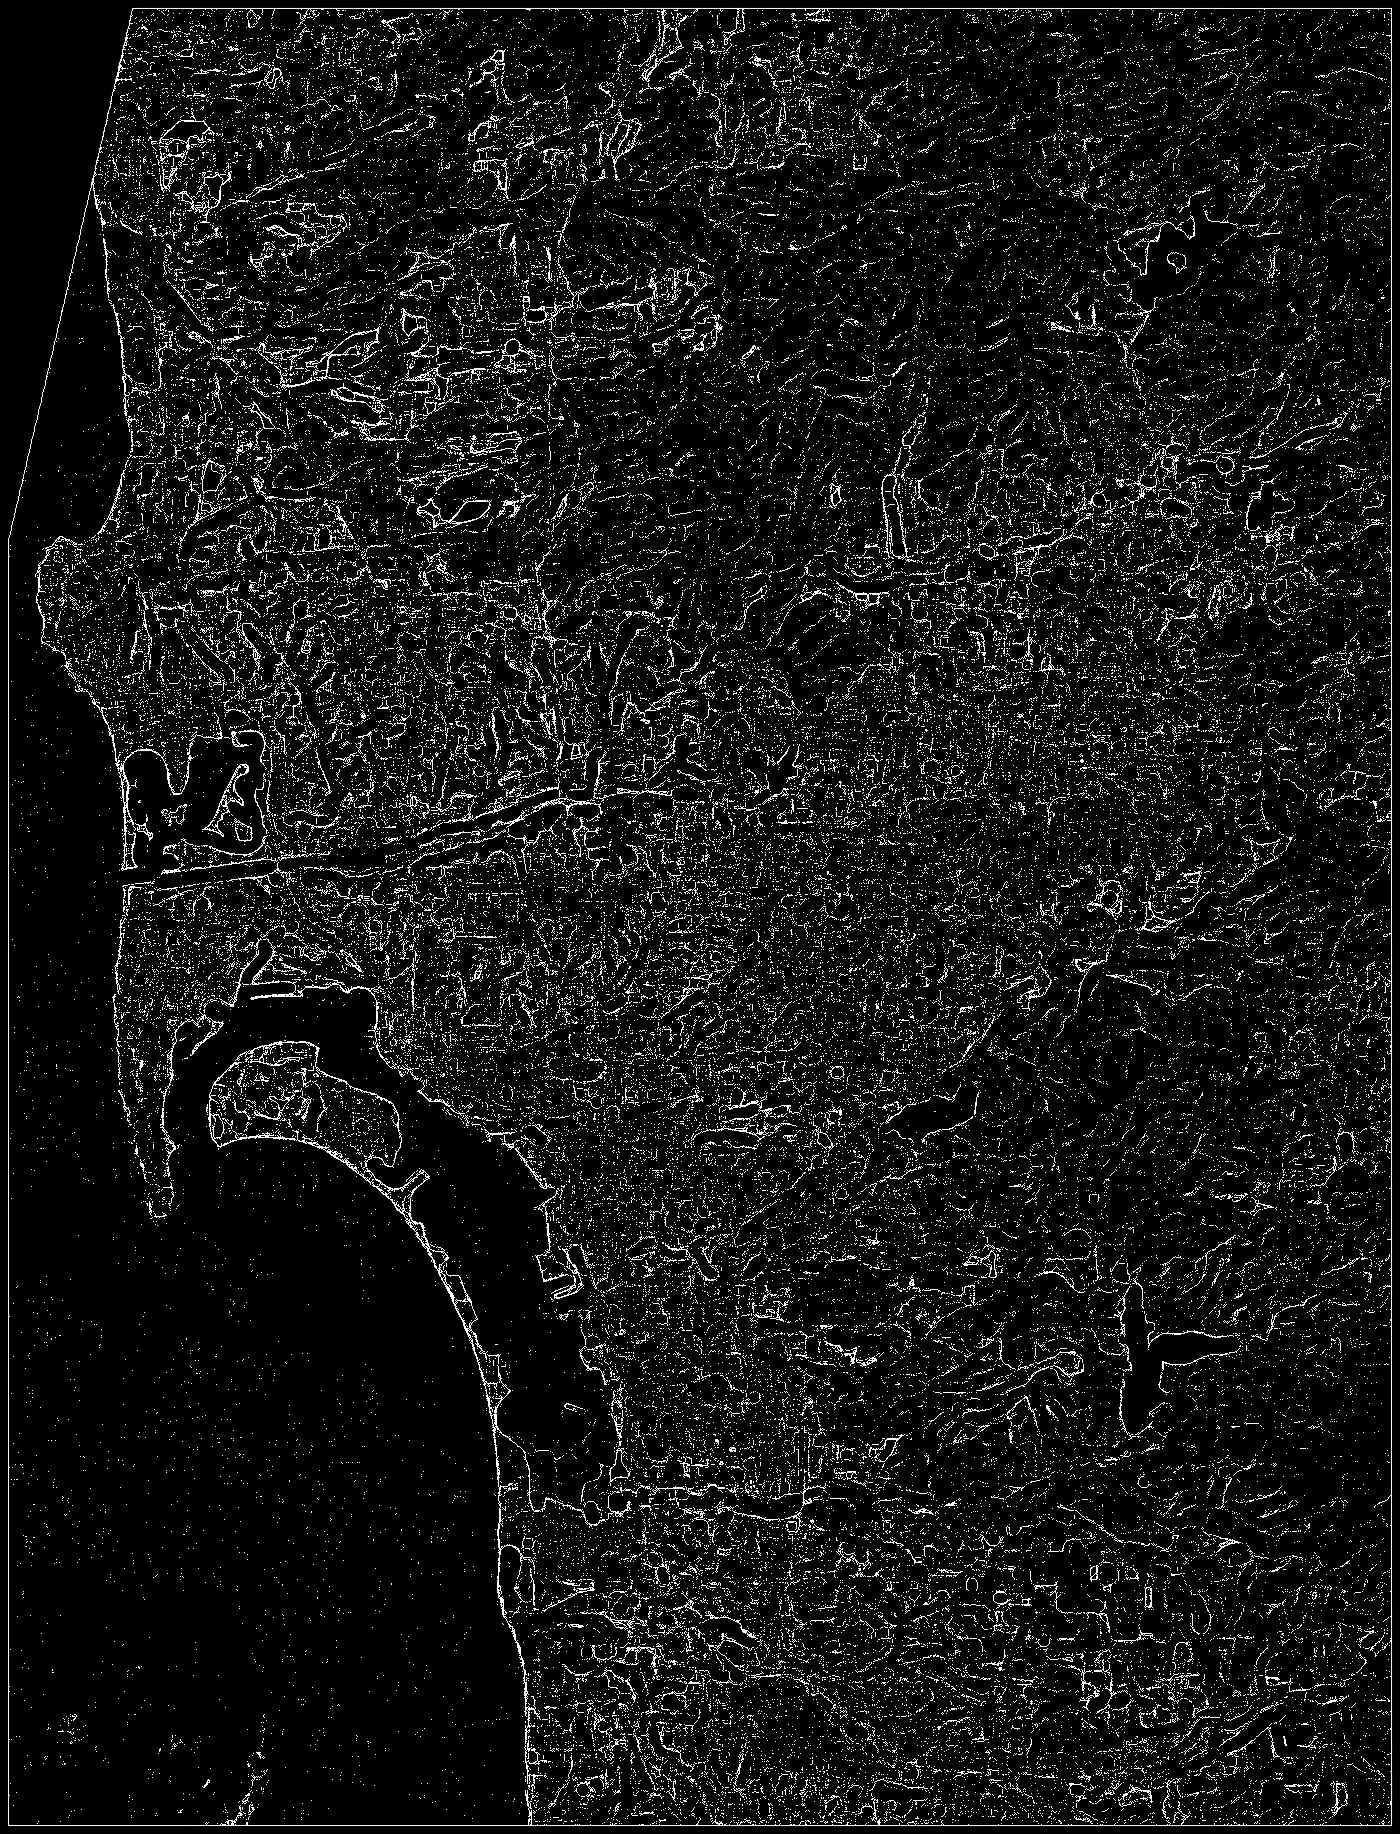
\includegraphics[width=12cm]{laplace2.png}
	\caption{A Laplace-szűrés eredménye egy medián szűrt űrfelvételre. A medián szűrés jelentősen mértékben eltüntette a zajokat, így az élek már sokkal világosabban látszanak}
	\label{fig:laplace2}
\end{figure}

\subsubsection{ConvolSingleBand}

Ez a függvény konvolúciós szűrést végez egy megadott frekvenciasáv intenzitásértékeit tartalmaz byte tömbre.

\subsubsection{Convol3bands}

Ez a függvény konvolúciós szűrést végez három megadott frekvenciasáv intenzitásértékeit tartalmaz byte tömbökre.

\subsubsection{highPassKernel}

Ez a függvény felül áteresztő kernelt számol.

\subsubsection{lowPassKernelGauss}

Ez a függvény alul áteresztő kernelt számol.

\subsubsection{lowPassKernelBox}

Ez a függvény alul áteresztő kernelt számol a box szűrőhöz.

\subsubsection{resampling}

Ez a függvény átmintavételezi az adott képet egy megadott mintavételi távolság alapján.

\subsubsection{Prewitt}

Ez a függvény Prewitt-féle éldetektálást végez.

\subsubsection{Sobel}

Ez a függvény Sobel-féle éldetektálást végez.

\subsubsection{Isotropic}

Ez a függvény Izotropikus éldetektálást végez.

\subsubsection{vectorize}

Ez a függvény raszteres kép vektorizálását végzi.


\subsection{\textbf{GeoMultibandMethods} osztály eljárásai}


\subsubsection{RGB}

Képzeljünk el egy háromdimenziós koordináta rendszert (\ref{fig:rgb1}. ábra), ahol a három tengely a három alapszínnek felel meg. 

\begin{figure}
	\centering
	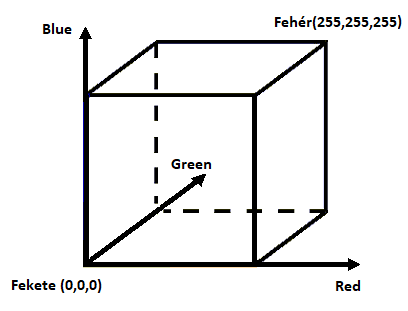
\includegraphics[width=7cm]{rgb1.png}
	\caption{Az RGB színkocka}
	\label{fig:rgb1}
\end{figure}  

Az RGB színmodell a színeket a vörös (Red), a zöld (Green) és a kék (Blue) alapszínek lineáris kombinációjaként állítja elő a következő módon:

\begin{equation} \label{formula:rgb}
Color = a \cdot Red + b \cdot Green + c \cdot Blue
\end{equation}


ahol $a,b,c$ együtthatók az egyes alapszínek részaránya az adott színben. Alkalmazzuk erre az esetre a 24 bites színmodellt. $2^{24}$féle színárnyalatot tudunk megjeleníteni, ami azt jelenti, hogy $2^8$ vörös, $2^8$ zöld és $2^8$ kék árnyalat jeleníthető meg, vagyis alapszínenként 256 fényerősség érték adható meg.

Egy adott frekvenciasáv intenzitás értékeit egy byte tömbben tároljuk, és egy RGB kép egy bitmappel reprezentálható, így három byte tömb alapján a bitmap kiszámolható, ha szükséges, meg is jeleníthető.

Definíciója a következő: 
\small
\begin{verbatim} Bitmap createRGB(byte[] byInR, byte[] byInG, byte[] byInB, int width, 
int height) \end{verbatim}

\subsubsection{NDVI}

Az NDVI (Normalized Difference Vegetation Index) szavakból alkotott mozaikszó, amely egy adott terület vegetációs aktivitását fejezi ki. A növényzet által visszavert fény intenzitásából számolható ki a következő módon: a közeli infravörös (NIR) és a látható vörös (RED) intenzitásainak különbsége és ezek összegének hányadosa szolgáltatja.

$$NDVI = \frac{NIR - RED}{NIR + RED} $$

A NDVI szoros összefüggést mutat a területet fedő növényzet fajlagos klorofill tartalmával. Így az egészséges növény más NDVI értéket mutat, mint a beteg vagy már halott (lásd \ref{fig:ndvi0}. és \ref{fig:ndvi1}. ábrák).
Definíciója a következő: 
\begin{verbatim} byte[] NDVI(byte[] bNIR, byte[] bIR) \end{verbatim}

\begin{figure}
	\centering
	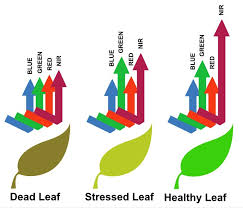
\includegraphics[width=7cm]{ndvi0.jpg}
	\caption{A különböző hullámhosszú fénysugarak visszaverődése különböző állapotú növényekről}
	\label{fig:ndvi0}
\end{figure}

\begin{figure}
	\centering
	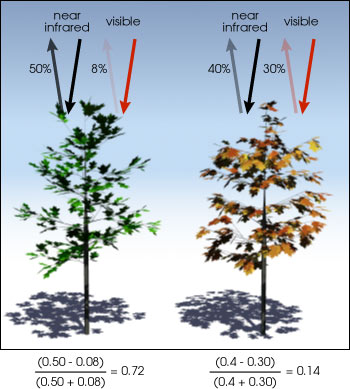
\includegraphics[width=6cm]{ndvi1.png}
	\caption{Az egészséges és a beteg növény viselkedése}
	\label{fig:ndvi1}
\end{figure}



\begin{figure}
	\centering
	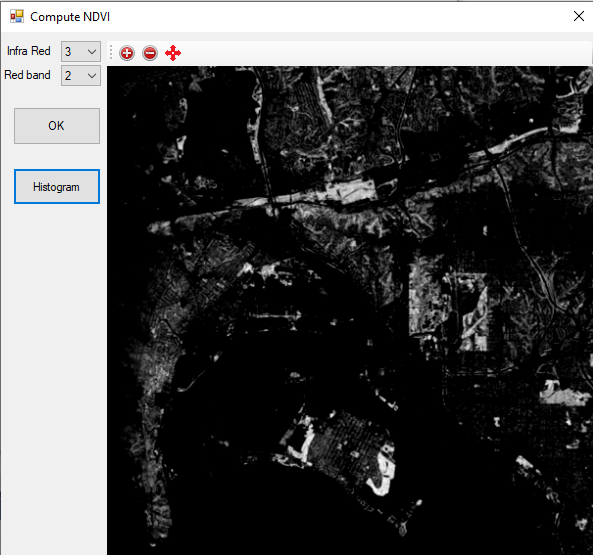
\includegraphics[width=10cm]{ndvi_pelda.png}
	\caption{Egy példa az NDVI-ra. A sötét területek a nem növényekkel fedett területeket mutatják (épületek, kopár talajfelszín, víz, stb.), míg a világos területek a növénnyel fedett részeket. Minél világosabb egy terület annál dúsabb rajta aa vegetáció}
	\label{fig:ndvi_pelda}
\end{figure}



\subsubsection{Cross Plot}

Az a függvény arra szolgál, hogy összehasonlítsuk két tetszőleges frekvenciasáv intenzitás értékeit. Az X-tengelyen az egyik, az Y-tengelyen a másik frekvenciasáv értékeit jelenítjük meg, ahogy azt a \ref{fig:crPlot}.  ábrán láthatjuk.

\begin{figure}
	\centering
	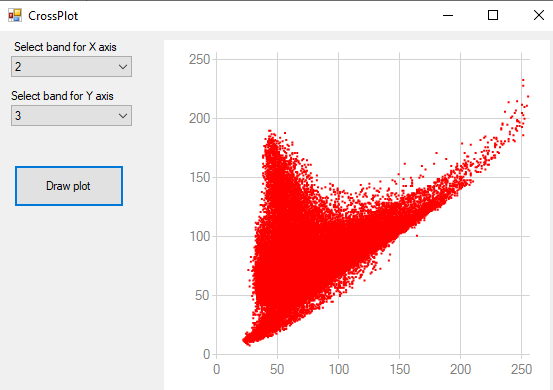
\includegraphics[width=10cm]{crPlot.png}
	\caption{Egy példa két különböző frekvenciasáv intenzitásainak összehasonítására}
	\label{fig:crPlot}
\end{figure}



\subsubsection{compEigen}

Kiszámítja egy megadott mátrix sajátértékeit és sajátvektorait.

\subsubsection{compPCA}

Ez a függvény kiszámítja a megadott byte tömbök által tárolt frekvenciasávok főkomponenseit. A \ref{fig:pca_landsat}. ábrán egy Landsat kép hét frekvenciasávjából számított első főkomponens látható.

\begin{figure}
	\centering
	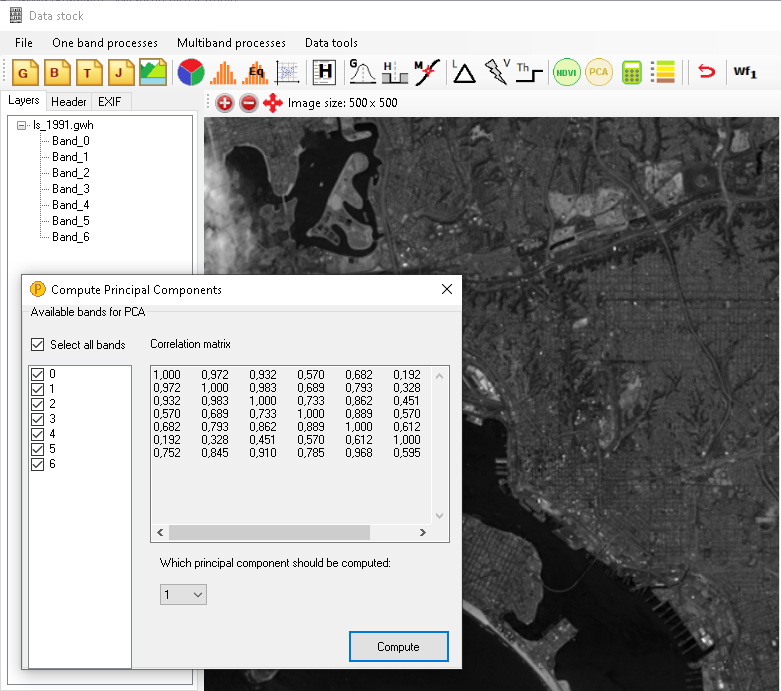
\includegraphics[width=12cm]{pca_landsat.png}
	\caption{Példa egy hét frekvenciasávból álló Landsat kép első főkomponensére}
	\label{fig:pca_landsat}
\end{figure}

\subsubsection{Clustering}

Az klaszterezési/osztályozási eljárások számos változata létezik. A \textit{Giwer} rendszer saját osztályozó eljárást fog alkalmazni, amely egy előzetesen végrehajtott szegmentálás eredményén fog dolgozni. Az osztályozás a szegmensekre kiszámított értékekre fog történni.

\subsubsection{Segmentation}

Számos szegmentálás eljárás létezik. A \textit{Giwer} rendszer egy éldetektáláson alapuló szegmentálási eljárást fog használni, amely elsődleges élek detektálása után, azok további szelekciójával fog előállítani szegmenshatárokat. A szegmensek értékei ezeken a határokon belüli pixelek értékei alapján lesznek kiszámítva.

A következőkben ismertetjük az eljárás elvi alapjait. Szegmenshatár ott van, ahol az intenzitás értékében markáns változás van. Tekintsük a legnagyobb intenzitásváltozás helyét a szegmens határának. Erre látunk példát a  \ref{fig:seg1}.  ábrán. Az a kék vonal azokat helyeket mutatja, ahol az eljárás szegmenshatárt detektált. 

Nemcsak a szegmenshatárok érdekesek a számunkra, hanem az intenzitásértékek is, amelyeket a szegmensekhez hozzárendelünk. Egy szegmensen belül homogénné tesszük az intenzitásokat, vagyis egy a szegmensre jellemző intenzitásértéket rendelünk hozzá. Jelen esetben azt a logikát követtük, hogy legyen a szegmens értéke a két szegmenshatár közötti értékek extremuma, ha ezek a szegmenshatárokon belülre esnek. Ha az extremumok a széleken vannak, akkor legyen a jellemző érték a határok közötti értékek átlaga.

\begin{figure}
	\centering
	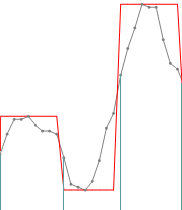
\includegraphics[width=5cm]{seg1.png}
	\caption{Az ábrán egy szintetikus adatsor (szürke görbe) intenzitásváltozásait láthatjuk egy dimenziós esetben. A szegmens határok ott vannak, ahol két csúcs között a legnagyobb az intenzitásváltozás. A kék vonal a szegmensek határait mutatja, a piros görbe pedig a szegmensekre kiszámított intenzitásértékeket. A szürke görbén lévő pontok az adatpontokat jelölik. }
	\label{fig:seg1}
\end{figure}

A \ref{fig:seg2}. ábrán egy SPOT kép szegmenshatárait láthatjuk. Ezek a határok a fent ismertetett inflexiós pont keresés alapján lettek megállapítva.

\begin{figure}
	\centering
	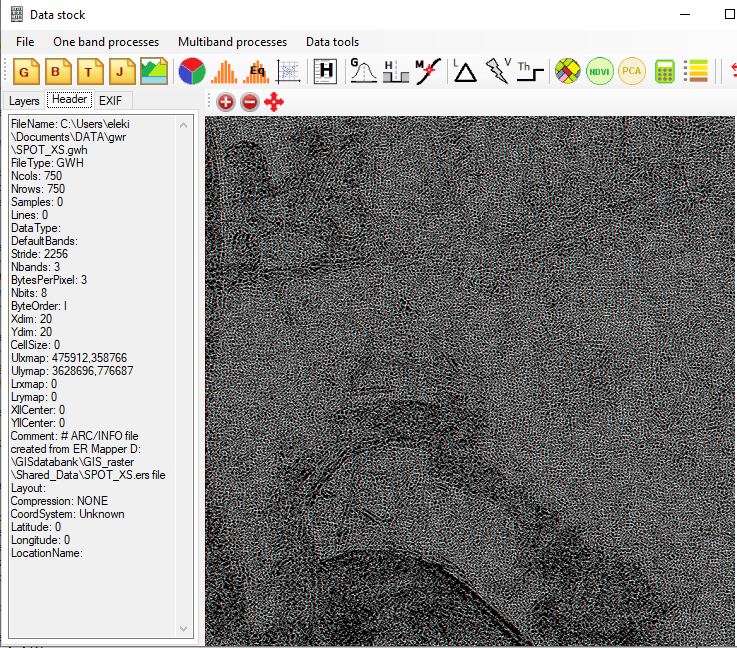
\includegraphics[width=14cm]{seg2.png}
	\caption{Az ábrán egy SPOT kép elemi szegmenshatárait láthatjuk. A kép azért furcsa, mert az eredeti képet EXOR művelettel kombináltuk össze a szegmenshatárokat tartalmazó képpel, vagyis, ahol nincs szegmenshatár, ott az eredeti képet láthatjuk, ahol viszont van határ, ott a határt láthatjuk }
	\label{fig:seg2}
\end{figure}



\subsection{A \textbf{DTM} osztály}

A digitális domborzatmodellre (DTM: digital terrain modell) egy külön osztályt hoztunk létre, mivel az adatok természete jelentősen eltér a képekétől. Minden DTM két byteon tárol egy magasság adatot, ugyanis egy byte 256 értéket képes csak tárolni, ami a magassághoz nem elegendő, mivel a Földön a magasságértékek -200 -- 8848 m között változnak. Két belső eljárása van, és egy propertyje, amely egy kétdimenziós tömb a magasságadatokkal.

A domborzat megjelenítésben is fontos, hogy ne csak greyscaleben, hanem valamely konvencionális megjelenési stílusban (pl. hipszometrikusan) is meg tudjuk jeleníteni az adatokat. 

\begin{figure}
	\centering
	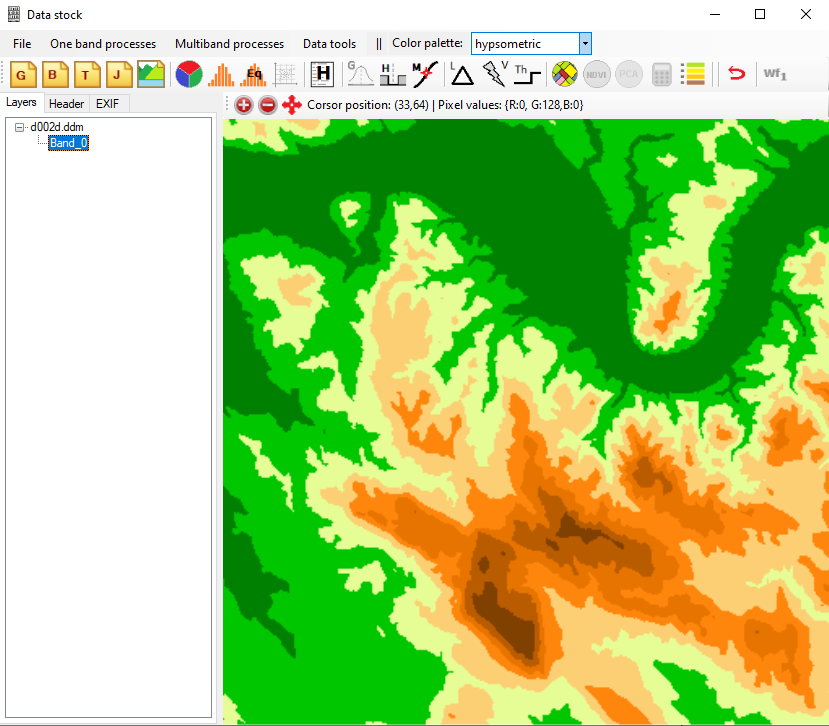
\includegraphics[width=14cm]{hipszo.png}
	\caption{A Dunakanyar hipszometrikusan megjelenített képe. A zöld szín a legalacsonyabb, a sötétbarna a legmagasabb területeket mutatja}
	\label{fig:hipszo}
\end{figure} 

\subsubsection{readParameters}

Ez az eljárás kiolvassa a DDM header fájljának tartalmát, és betölti a megfelelő propertykbe. A fájlnév megadásakor hívódik meg.

\subsubsection{readDDM}

Ez az eljárás beolvassa az adatsor paraméterivel leírt magasság adatokat egy kétdimenziós tömbbe, amelyet tárol a megfelelő propertybe. A readParameters eljárás után hívódik meg.

\subsection{A \textbf{Raster Calculator} osztály}

A \textbf{Raszter calculator} osztálynak egyelőre két fő funkciója van, amelynek paramétereit a felhasználó állíthatja be, amint a \ref{fig:rastcalc1}. ábrán látható.

\begin{itemize}
	\item Where feltételként egy értéket adhatunk meg összehasonlításra
	\item Where feltételként két értéket (between) adhatunk meg összehasonlításra
\end{itemize}
	
\begin{figure}
	\centering
	\includegraphics[width=12 cm]{rastcalc1.png}
	\caption{Az ábrán a \textbf{Raster calculator} kommunikációs felületét láthatjuk }
	\label{fig:rastcalc1}
\end{figure}	

\subsection{A \textbf{Project} osztály}

A \textbf{project} osztálynak egy eljárása van, a \textit{loadProjectFile}, amely betölti projectben lévő képek fájljait a \textit{FileNames} nevű listába. A későbbiekben ez a gyűjtemény akkor is jól használható lesz, ha ugyanazt az eljárást, vagy egy workflowt kívánunk lefuttatni a projekt összes fájljára.

Különösen akkor válik ez igen hasznossá, ha sok drón felvételből kívánunk egy mozaik képet létrehozni.


\section{A DataStock alrendszer használata}

A \textbf{Giwer} rendszer interaktív modulja a \textbf{DataStock}, ami a menürendszeren keresztül teszi elérhetővé a függvénykönyvtárat és az adatokat. Különböző típusú grafikus fájlok (\textit{bil, tif, jpg}) beolvasását és manipulálását végzi. Speciális, saját fájlformátuma a \textit{GWR/GWH} formátum. A \textit{GWH} egy header fájl, amely az adott kép metaadatait tartalmazza, míg a \textit{GWR} egy bináris formátum, amely egységesen kezelhetővé teszi a legkülönbözőbb forrásokból származó adatokat, és lényegesen gyorsabbá teszi a feldolgozási műveleteket.

\subsection{Menürendszer}

A menürendszer (\ref{fig:datastock_fomenu}. ábra) \textit{File}, \textit{One band processes}, \textit{Multiband processes} és \textit{Data tools} menüelemekből áll, valamint jelzi az aktuális \textit{Lookup table}-t mutatja (default, hypsometric, ndvi, user stb), amelyet szükség szerint átállíthatunk egy másikra. A \textit{default} beállítás greyscale megjelenítést végez. A \textit{hypsometric} egy 8 bites, maximum 256 színű színezést tesz lehetővé attól függően, hogy a \textit{lookup table}-ben hány színt állítottunk be. Ez a hagyományos hipszometrikus megjelenítés stílusa, amely az alacsony területeket a zöld árnyalataival, a kissé magasabb területek a sárga árnyalataival, és a magas területeket a barna árnyalataival jeleníti meg. Az \textit{ndvi} az ndvi számításkor használatos színes megjelenítést teszi lehetővé. A \textit{user} a felhasználó által beállított \textit{lookup table}-t állítja be.

\begin{figure}
	\centering
	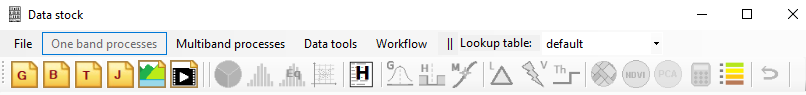
\includegraphics[width=14cm]{datastock_fomenu.png}
	\caption{A \textbf{datastock} fő menüje}
	\label{fig:datastock_fomenu}
\end{figure}

\subsubsection{File}

A \textit{File} menüvel (\ref{fig:filemenu_datastock}. ábra) meg tudunk nyitni \textit{gwh, bil, tif, jpg} típusú fájlokat, valamint projekt fájlokat, amelyek egyszerre több kép kezelésére szolgálnak. Törölhetjük valamely (akár több) \textit{gwh} fájlt. A \textit{gwh, gwr} fájlok a \textbf{Giwer} rendszer saját formátumú fájljai. Elmenthetjük egy feldolgozás eredményét giwer formátumban, vagy egyszerű bitmapként. Elmenthetjük továbbá projektként is a \textbf{Giwer}-ben lévő adatoknak azt az állapotát, ami egy adott pillanatban éppen fennáll. Végül pedig ismételten betölthetjük a rendszer konfigurációs adatait, ha időközben megváltoztattuk azt a keretprogrammal (nem frissül automatikusan).

\begin{figure}
	\centering
	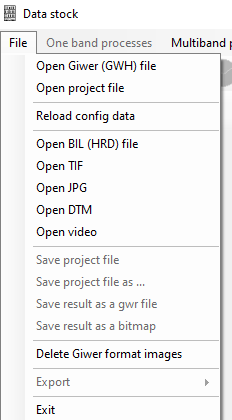
\includegraphics[width=4cm]{filemenu_datastock.png}
	\caption{A \textbf{File} menü}
	\label{fig:filemenu_datastock}
\end{figure}

A képek beolvasása még nem jelent megjelenítést. Ehhez ki kell választanunk a megjeleníteni kívánt frekvenciasávot a \textit{Data stock} ablak \textit{Layers} fülén lévő valamelyik listaelemre kattintással (\ref{fig:layer_list}. ábra). A kiválasztás után a legtöbb menüelem és gyors gombok (főmenü alatti ikonok) aktív állapotba kerülnek.

\begin{figure}
	\centering
	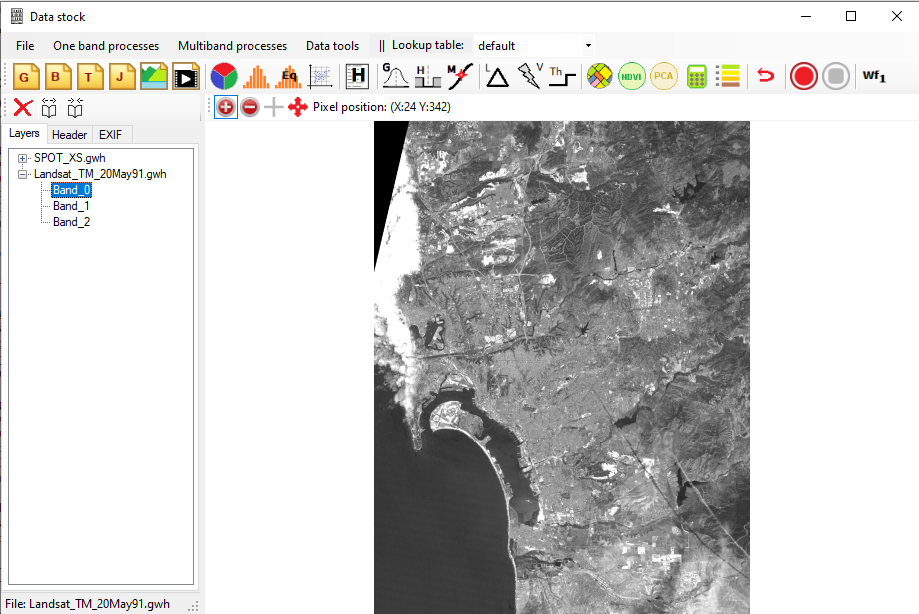
\includegraphics[width=14cm]{layer_list.png}
	\caption{Képek megjelenítése a \textit{Layer list} valamely elemének kiválasztásával}
	\label{fig:layer_list}
\end{figure} 

A \textit{gwh} egy text fájl, amely header tipusú adatokat tartalmaz a képről (szélesség, magasság, frekvenciasávok száma, bitmélység, stb.), míg a \textit{gwr} egy bináris fájl, amely pixeladatokat tartalmaz sorfolytonosan. 

A \textit{bil} fájl egy régi űrfelvétel formátum, amely szintén header fájlból és egy bináris fájlból áll. A *.hdr fájl a kép metaadatait, *.bil pedig a pixel adatokat tartalmaz. Részletes leírása megtalálható a \newline \textit{http://desktop.arcgis.com/en/arcmap/10.3/manage-data/raster-and-images/ bil-bip-and-bsq-raster-files.htm} weboldalon. 

A \textit{tiff, jpg} fájlok jól ismert képformátumok, amelyek különböző színmélységű és sávszámú képek tárolására alkalmasak.

A menüsor alatti ikonosztázon (gyors gombok) láthatók a leggyakoribb fájltípusok megnyitására szolgáló ikonok, mint \includegraphics[width=0.5cm]{opengiwer.png} (open giwer format), \includegraphics[width=0.5cm]{openbil.png} (open bil format), \includegraphics[width=0.5cm]{opentif.png} (open tif format), \includegraphics[width=0.5cm]{openjpg.png} (open jpg format), 
\includegraphics[width=0.5cm]{3d.png} (open 3D) és \includegraphics[width=0.5cm]{openvideo.png} (open video).


\subsubsection{One band processes}


Ez a menü akkor használható, amikor egy kiválasztott frekvenciasávval kívánunk műveleteket végrehajtani. Kiválasztás után meg is jelenik a képablakban. %(\ref{fig:ug_datastock2}. ábra).
A \textit{One band processes} menü elemei a következők: \textit{Histogram, Thresholding, Vecorizing, Filters, Texture, Segmentation, Clustering, Raster calculator} (\ref{fig:onebandmenu}. ábra).

\begin{figure}
	\centering
	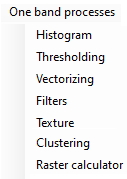
\includegraphics[width=4cm]{onebandmenu.png}
	\caption{A \textbf{One band processes} menü}
	\label{fig:onebandmenu}
\end{figure}

\begin{itemize}
	
	\item A \textit{Draw histrogram} almenü kirajzolja a kép hisztogramját, amelyet a kép kiegyenlítésére (kontrasztosítására) használhatunk. A bal egérgomb klikkel a minimális, a jobb egérgomb klikkel a maximális értéket választhatjuk ki. Az \textit{Equalize} gombbal elvégezzük a kiegyenlítést. 
	%	Választhatjuk a \textit{Histrogram equalization} gombbal, hogy automatikusan választjuk ki a minimális és maximális értéket, és hajthatjuk végre a kiegyenlítést. Ilyenkor a hisztogram nem rajzolódik ki, csak az eredmény a képen.	
	%	
	\item Ha a \textit{Histrogram equalization} menüre kattintunk, akkor automatikus választjuk ki a minimális és maximális értéket, és hajthatjuk végre a kiegyenlítést. Ilyenkor a hisztogram nem rajzolódik ki, csak az eredmény a képen.
	
	\item A \textit{Thresholding} küszöbölést hajt végre egy megadható küszöbértéktől függően. Általában más eljárásokkal kombinálva használható.
	
	\item A \textit{Vectorizing} vektoros jellegű adatot állít elő a képből. A nyers képre nem érdemes alkalmazni, mert az eredmény rossz lesz. Mielőtt alkalmaznánk, előtte simítószűrést, küszöbölést és éldetektálás (Laplace filter) kell végezni. 
	
	\item A \textit{Filters} egy több almenüből álló gyűjtemény, amely különböző szűrési eljárásokat (\textit{Gauss smoothing, High pass filter, Gradient filters, Laplace filter, Median filter}) végez a képen. 
	
	\item A \textit{Texture} menü az aktuális kép textúráját elemzi (fejlesztés alatt)
	
	\item A \textit{Segmentation} menü az aktuális frekvenciasáv szegmentálását végzi.
	
	\item A \textit{Clustering} menü az aktuális frekvenciasáv  osztályozását végzi.
	
	\item A \textit{Raster calculator} menü leválogatja az aktuális frekvenciasáv azon pixeljeit, amelyek a megadott  feltételeket eleget tesznek.
	
	
\end{itemize}


\subsubsection{Multiband processes}

A\textit{ Multiband processes} csoportba azok a funkciók tartoznak, amelyek egyszerre több frekvenciasáv adatait igénylik mint pl. RGB képek létrehozása, PCA (főkomponens analízis a megadott frekvenciasávokra), NDVI (vegetációs index), több frekvenciasáv alapján történő osztályozás, képek kombinálása (\ref{fig:multiband_menu}. ábra). 


\begin{figure}
	\centering
	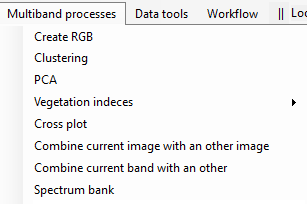
\includegraphics[width=5cm]{multiband_menu.png}
	\caption{A \textit{Multiband processes} menü}
	\label{fig:multiband_menu}
\end{figure}


\begin{itemize}
	
	\item A \textit{Create RGB} menü RGB képet kreál a megadott három frekvenciasávból
	
	\item A \textit{Segmentation} menü a kiválasztott frekvenciasávokra szegmentálást végez.
	
	\item A \textit{Clustering} menü a kiválasztott frekvenciasávokra osztályozást végez.
	
	\item A \textit{PCA} menü a kiválasztott frekvenciasávokra főkomponens analízist végez
	
	\item Az \textit{NDVI} menü a kiválasztott frekvenciasávokból vegetációs indexet számol.
	
	\item A \textit{Cross plot} menü a kiválasztott két frekvenciasávból cross plottot rajzol.
	
	\item A \textit{Combine current image with...} az aktuális képet kombinálja (+,-, EXOR) egy tetszőleges másik képpel. Ez olyankor hasznos, ha például egy vektorizált képet össze akarunk rajzolni az eredeti képpel (ekkor az EXOR operátort kell használni).
	
	
\end{itemize}

\subsubsection{Data tools}

A \textit{Data tools} menü az adatok előkészítésére való funkciókat tartalmazza (\ref{fig:datatools_menu}. ábra). Különböző formátumok konverzióját, egyesítését, kombinálást végzi. Néhány a drón képekkel kapcsolatos problémát old meg. A \textit{Lookup table} szerkesztését is lehetővé teszi. Legfontosabb funkciója azonban a \textit{Convert to Giwer format} almenü. Ennek segítségével bármely nyers képformátumot (bil, tif, jpg) giwer formátumba konvertálja. 

A giwer formátum kétféle fájlt jelent: a \textit{.gwr} egy bináris fájl, ami a képet tartalmazza frekvenciasávonként, a \textit{.gwh} pedig a kép header információit tartalmazza.

\begin{figure}
	\centering
	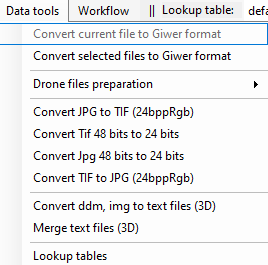
\includegraphics[width=5cm]{datatools_menu.png}
	\caption{A \textit{Data tools} menü}
	\label{fig:datatools_menu}
\end{figure}


A \textit{Convert to Giwer format} menü csak akkor aktív, ha a \textit{Layers} fül listáján valamely tif, jpg vagy bil formátumban lévő kép ki van választva. Erre a menüre kattintva végrehajtódik a konverzió, és a \textit{Config} fájlban megadott helyre (GiwerDataFolder) képződik a konvertált adat. Ezután ezt a fájlt megnyitva a \textit{Data Stock} teljes funkcionalitása rendelkezésre áll. A többi formátumú kép számára a feldolgozó műveletek nem aktivizálhatók, csak a \textit{giwer} formátumúakra.

A \textit{Drone files preparation} menü bizonyos képek megfelelő formátumba hozására szolgál. A Micasense multispektrális kamera, amelyeknek 3 RGB, és 2 infravörös sávja, valamint egy termális sávja van, annyi tif fájl állít elő, ahány sávja van, jelen esetben 6 db tif fájlt. Ha ezeket szeretnénk gwr formátumba konvertálni, akkor két lehetőségünk van, amit két almenü tesz lehetővé:
\begin{itemize}
	\item A \textit{Merge multiple images to giwer format} menüre kattintva megjelenik egy dialógus ablak, ahol kiválaszthatjuk a kérdéses fájlokat. Ezután elindul a konverziós folyamat, amelynek eredményeként egy db \textit{GWH} fájl és 6 db \textit{GWR} fájl keletkezik. A header egy 6 sávos képet fog leírni. Mindenképpen ez a módszer ajánlható, mert a \textit{Multiband processes} feldolgozási folyamatok csak ilyen fájlokra működnek.
	
	\item A \textit{Convert each multiple image to giwer format} menüre kattintva megjelenik egy dialógus ablak, ahol kiválaszthatjuk a kérdéses fájlokat. Ezután elindul a konverziós folyamat, amelynek eredményeként 6 db \textit{GWH} fájl és 6 db \textit{GWR} fájl keletkezik. Így minden egyes sáv egysávos képnek fog látszani. Ezekre csak a \textit{One band processes} menü funkciók fognak működni.
\end{itemize}

\subsubsection{Néhány hasznos funkció}

A főbb funkciócsoportok után néhány apróbb, inkább kényelmi funkciót is ismertetünk. A menüsor alatt található egy ikonosztáz, amely a menürendszerből bizonyos funkciókat gyorsabban elérhetővé tesz:\\

\includegraphics[height=0.55cm]{ikonosztaz.png} \\Balról jobbra a következő funkciók érhetők el: gwr, bil, tif, jpg és video fájlok megnyitása, RGB kép készítése, kétféle hisztogram művelet, ahol az első interaktív, és meg is jelenízi a hisztogramot, a másik automatikus. Cross plot rajzoló két frekvenciasáv adatait jeleníti meg egy grafikonon. A \textbf{H} feliratú ikon a header adatok elrejtését/megjelenítését végzi. 

A G ikon Gauss-simítást, a H a high pass filter indítja, az M a medián szűrést, az L a Laplace szűrést, a Th a thresholdingot. Ezután jön az osztályozás ikonja, majd az NDVI számítóé, a főkomponens analízisé (PCA), majd a raszter kalkulátor, és végül a Lookup table szerkesztő. A piros vissza-nyíl \textit{undo} funkció, vagyis visszaállítja az utolsó művelet előtti állapotot (csak egy visszalépés lehetséges). A nagy piros gombok a workflow editáláshoz használatosak.

A \textit{Layers} fülön három ikon van: 
\includegraphics[height=0.55cm]{layer_list_icons.png}. A piros kereszt törli az egész layer listát. A kinyíló könyv az összes listán lévő kép frekvenciasávjainak listáját kinyitja, míg a bezáródó könyv bezárja őket. Ha csak egyetlen elemet akarunk törölni a listáról, akkor a jobb egérgombbal klikkeljünk a kívánt listaelemre, és a felbukkanó menüből válasszuk ki a törlést.



\section{A Catalog alrendszer használata}

A \textbf{Catalog} alrendszer nagy tömegben keletkező képek (csak \textit{jpg} és \textit{tif} formátumú képek) rendszerezésére, adatbázisba szervezésére való (ehhez sqlite-ot használ a program). Az adatok és a képek gyors szemrevételezését is lehetővé teszi. A \textbf{DataStock} alrendszer használata enélkül is lehetséges, hiszen bármely képet használatba vehetjük vele. A \textbf{Catalog}ot olyankor célszerű használni, amikor több száz vagy több ezer képet kívánunk egységesen kezelni, a leíró adataik alapján keresést végezni.

\subsection{Első lépések}

\begin{itemize}
	\item Másoljuk be egy könyvtárba a catalog.zip fájlt.
	\item Bontsuk ki.
	\item Ahová kibontottuk, onnan indítható a catalog.exe, nem kell külön telepíteni.
	\item Az első induláskor még nincs képi adatbázis, ezért panaszkodni fog a hiányára (\ref{fig:missingdb}. ábra):
	
	\begin{figure}[h]
		\centering
		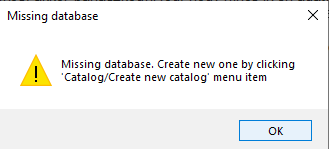
\includegraphics[width=8cm]{missingdb.png}
		\caption{A 'Missing database' üzenet}
		\label{fig:missingdb}
	\end{figure}
	
	\item Ezután megjelenik a program fő formja, ahol kreálhatunk egy új, üres adatfájl (\ref{fig:createnewcatalog}. ábra) (a default név 'dronimagecatalog.s3db', de lehet bármi más is)
	
	\begin{figure}
		\centering
		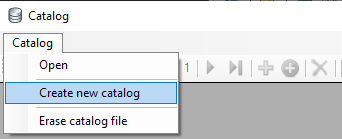
\includegraphics[width=8cm]{createnewcatalog.png}
		\caption{A \textit{Create new catalog} menü}
		\label{fig:createnewcatalog}
	\end{figure}
	
	\item Ezután a 'Open' menüre klikkelve megnyílik az üres adatbázis-fájl.
	
	\item Ha már van létező adatbázis (pl. dronimagecatalog néven), akkor megjelenik a tartalma egy táblázatban a program fő formján (\ref{fig:catalog0}. ábra). Ritka eset, de ha nincs, akkor panaszkodni fog, hogy nincs ilyen adatbázis  –- mert például kitörültük a fájlrendszerből, de a catalog még úgy emlékszik, hogy van ilyen fájl. Kattintsunk az OK-ra, majd nyomjuk meg az F2 gombot -– bal felső sarok környéke a billentyűzeten. Ekkor megjelenik egy 'Catalog' nevű menü. Válasszuk ki a 'Create new catalog' almenüt, amely létrehoz egy 'dronimagecatalog' nevű adatbázist, és benne egy üres adattáblát, amelynek 'images' lesz a neve. Ide fognak képződni a felvett képek adatai.
	
	\begin{figure}
		\centering
		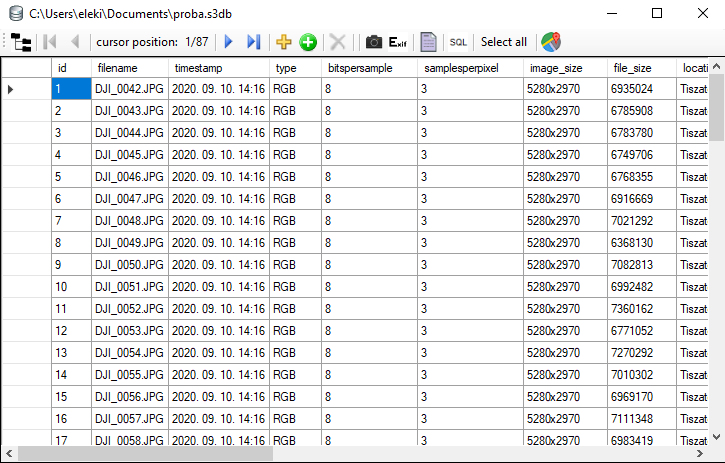
\includegraphics[width=13cm]{catalog0.png}
		\caption{A \textit{Catalog} fő formja}
		\label{fig:catalog0}
	\end{figure}
	
	\item Normál indulásnál a menürendszer nem látszik (F2-t megnyomva jelenik meg és tűnik el)
	
	\item Az ikonok elmondják, hogy mit tudnak, ha az egeret föléjük mozgatjuk.
	
\end{itemize}

\subsection{A fájlrendszer előkészítése}

\begin{itemize}
	\item Kreáljunk egy könyvtárat 'DRON\_IMAGES' néven valahol a fájlrendszerben.
	
	\item Klikkeljünk az 'open folder tree' ikonra (
\includegraphics{open_folder_structure.png}). Ekkor megnyílik a 'Folder structure' nevű ablak (\ref{fig:folder_struc}. ábra).
	
	\item Klikkeljünk a 'Set destination folder' nevű menü gombra, majd keressük meg és válasszuk ki a 'DRON\_IMAGES' nevű könyvtárat. Ezzel megadtuk a kép katalógus helyét a fájlrendszerben, amire ezentúl emlékezni fog a program, ha újra megnyitjuk a 'Folder structure' ablakot. 
	
	\item Keressük meg a flash driven-on (ami a dronon a képeket tárolja) azt a könyvtárat, ahol az éppen most készített képek vannak. Ha a jobb oldali ablakban megjelennek a fájlok, klikkeljünk a 'Save files to '\verb|c:\DRON_IMAGES| folder' ikonra (
\includegraphics{save.png}). Ennek hatására az egész könyvtár tartalma átmásolódik a flash driveról a 'DRON\_IMAGES' nevű könyvtárba.
	
	\item Ennek hatására a 'DRON\_IMAGES' nevű könyvtárban megjelenik egy új directory, aminek a neve az első fájl mentésének időpontja. Ez a könyvtár fogja tartalmazni az adott időben történt repülés képeit.
\end{itemize}

\begin{figure}
	\centering
	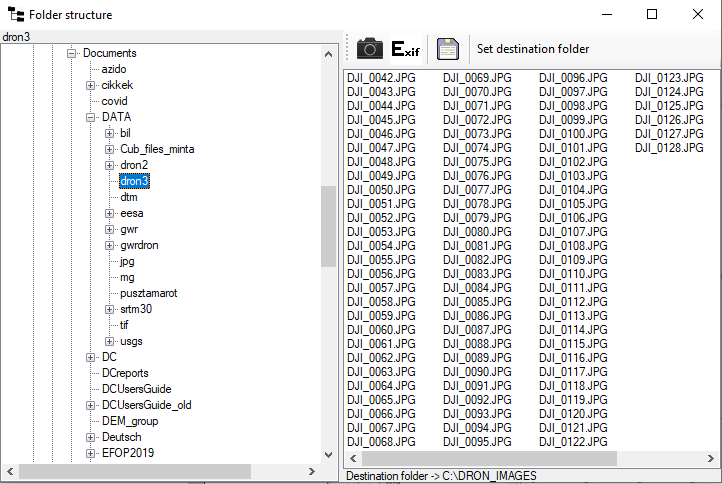
\includegraphics[width=13cm]{folder_struc.png}
	\caption{A \textit{Folder structure} ablak}
	\label{fig:folder_struc}
\end{figure}

\subsection{Az adatbázis feltöltése}

\begin{itemize}
	\item Kétféleképpen tölthetjük fel az adatbázist: vagy egyenként (vagy multiselecttel több fájlt is) vagy egy directory-t kijelölve tömegesen, annak teljes tartalmát (csak jpg és tif fájl, más nem). A fájlonkénti kijelöléshez klikkeljünk a sárga plusz jelre (
\includegraphics[width=0.5cm]{plus.png}), a teljes directory kijelöléséhez a zöld karikában fehér kereszt ikonra (
\includegraphics[width=0.5cm]{addfolder.png}).
	
	\item Bármelyikre klikkeltünk, felbukkan a 'Editable image attributes' nevű ablak (\ref{fig:editableimageattribute}. ábra), ahol megadhatjuk azokat az adatokat, amelyek minden most beemelendő képre vonatkoznak. A többi adatot a program automatikus feltölti (fájlnév, long, lat, timestamp, folder, stb.).
	
	\begin{figure}
		\centering
		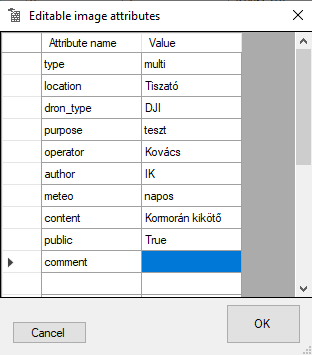
\includegraphics[width=6cm]{editableimageattributes.png}
		\caption{Az \textit{Editable image attributes} ablak}
		\label{fig:editableimageattribute}
	\end{figure}
	
	\item A táblázat nem automatikus adatai szerkeszthetők, amik el is mentődnek, amint a következő rekordra lépünk.
	
	\item A fényképezőgép ikonra 
\includegraphics[width = 0.5 cm]{camera.png}) kattintva megjelenik az aktuális rekordhoz tartózó kép. Az 'Exif' (
\includegraphics[width = 0.6 cm]{exif.png}) feliratú ikon az aktuális rekordhoz tartozó kép exif adatait mutatja meg egy külön ablakban.
\end{itemize}

\subsection{Funkciók}

Az adatokat mutató táblázat felett egy ikonosztáz látható, amelyen a főbb funkciók lettek elhelyezve. A 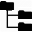
\includegraphics[width = 0.5 cm]{filesystem.png} ikon megnyit egy a fájlrendszert nézegető ablakot, hol megnézhetjük az adatok forrását, mint pl. egy pendrive-ot, ami közvetlenül a drón adattároló eszköze, és amelyen a legfrissebb mérési adatok vannak(\ref{fig:folder_struc}. ábra). A kiválasztott fájlokat (az egész könyvtárat) a \textit{DRON\_IMAGES} nevű könyvtárba másolja be. Amúgy ezt az első használat során meg kell adni (\textit{Set destination folder}). A másolást a 
\includegraphics[width=0.5cm]{save.png} ikonra való klikkelés végzi.

Az adatbázisban már bent lévő képeket a 
\includegraphics[width = 0.5 cm]{camera.png}  ikonnal, míg a hozzá tartozó EXIF adatokat az 
\includegraphics[width = 0.5 cm]{exif.png}  ikonnal nézhetjük meg.

Új képeket, egyenként a \includegraphics[width=0.5cm]{plus.png} ikonnal, míg tömegesen, vagyis egy egész directory tartalmát, a \includegraphics[width=0.5cm]{addfolder.png} ikonnal adhatjuk hozzá az adatbázishoz. A hozzáadás egyben az adatbázis feltöltését is elvégzi, persze csak azokat az adatokat, amelyek a képekből kinyerhetők. Interaktívan is hozzáadhatók adatok, ha azokat a megfelelő mezőbe beírjuk. A \includegraphics[width=0.5cm]{del.png} ikonnal egy kijelölt rekordot törölhetünk. Nemcsak a leíró adatok törlődnek (az 'images' nevű tábla kijelölt rekordja), hanem a \textit{DRON\_IMAGES} könyvtárból is a kijelölt kép fájl (UNDO nincs!).

\begin{figure}
	\centering
	\includegraphics[width=12cm]{sqleditor.png}
	\caption{Az \textit{Sql editor} ablak}
	\label{fig:sqleditor}
\end{figure}

Az \includegraphics[width=0.5cm]{sql.png} ikonnal SQL parancsokat állíthatunk össze, amelyekkel tetszőleges feltétel szerint kereshetünk (legyűjthetünk) a rendelkezésre álló képek paraméterei alapján. Az \ref{fig:sqleditor}. ábrán olyan képek legyűjtésének eredménye látható, amelyek a Tiszán készültek, és a kép típusa 'multispektrális'. Az 'Sql editor' az Sql-t nem, vagy csak alapszinten ismerők számára is használható. 
(Az Sql-ben járatos felhasználók számára előhívható egy rejtett Sql parancssor, amely azért rejtett, mert hozzá nem értők kezében veszélyes fegyver lehet, amellyel súlyos károkat is lehet okozni az adatbázisban. Akik biztosak az Sql tudásukban, azok az F12 gomb megnyomásával előhívhatják az Sql parancssort, amely eltüntethető, ha újra megnyomjuk az F12 gombot. Nemcsak lekérdező, hanem non query típusú parancsok is kiadhatók. A parancs \textbf{Enter}rel hajtható végre.)


A \includegraphics[width = 0.5 cm]{sheet.png} ikonnal egy adott mérésre vonatkozó riport fájlt nézetünk meg, vagy hozhatunk létre, amelybe olyan adatokat tehetünk bele, amelyeket a mérési körülmények miatt, vagy bármilyen szempontból érdekesnek találunk, de nem az egyes képekhez kötöttek.

\subsection{Lekérdezés}

\begin{itemize}
	\item  Az 'SQL' feliratú ikonra klikkelve (\includegraphics[width=0.5cm]{sql.png}) megjelenik egy 'Query editor' nevű ablak. Itt ki lehet választani, hogy melyik mezőre kérdezünk, milyen feltételt szabunk.
	
	\item pl. select field: type;  Operator: =; Value: RGB ====> WHERE type=RGB. Ha itt vége, akkor click to 'Generate WHERE condition and Sql command' majd 'Execute query'. 
	
	\item Ha új lekérdezés lesz, akkor előtte click to 'Clear WHERE or new command'. Vigyázat, az Sql editor case sensitive (rgb !=  RGB)
	
	\item Összetettebb lekérdezésekhez az előbbihez hasonló lekérdezés után klikkeljünk az 'Add further condition' nevű check boxra. 
	
	\item Ha kész vagyunk egy further feltétellel, klikkeljünk az 'Add further condition'- gombra. Ha az utolsót is hozzáadtuk, akkor klikkeljünk a 'Generate WHERE condition and Sql command' majd az 'Execute query'-re. Ha jó volt az sql parancs, akkor megjelenik az eredmény az adatrácsban.
	
	\item Ha meg vagyunk elégedve az eredménnyel, klikkeljünk a 'Close and return to main window' gombra. Ekkor becsukódik a 'Query editor' ablak, és a lekérdezés eredménye megjelenik a fő ablakban. Itt nézegethetjük a képek listáját.
	
	\item A 'Select all' feliratú gombra a bal egérgombbal klikkelve az összes képet legyűjthetjük az adatbázisból, amelyek adatai meg is jelennek az adatrácsban.
	
	\item A 'Select all' feliratú gombra a jobb egérgombbal klikkelve az összes képet kijelölhetjük az  adatrácsban (\ref{fig:mapviewer_select_all}. ábra). Ezt olyankor hasznos, amikor térképen akarjuk megjeleníteni a legyűjtött képek centroidjait. Ehhez még rá kell kattintani a \includegraphics[width = 0.5 cm]{mapviewer_ikon.png} ikonra. Ekkor megjelennek a 'Map viewer' ablakban (\ref{fig:mapviewer}. ábra felső része) a képek centroidjai. Ha úgy klikkeltünk a \includegraphics[width = 0.5 cm]{mapviewer_ikon.png} ikonra, hogy nem jelöltünk ki egyetlen képet sem, akkor az ELTE Térképtudományi és Geoinformatikai Intézet helye jelenik meg a térképen (a \ref{fig:mapviewer}. ábra alsó része).
	
	\begin{figure}
		\centering
		\includegraphics[width=12cm]{mapviewer_select_all.png}
		\caption{A \textit{Map viewer} ablak}
		\label{fig:mapviewer_select_all}
	\end{figure}
	
	\begin{figure}
		\centering
		\includegraphics[width=12cm]{mapviewer.png}
		\includegraphics[width=12cm]{tegeta.png}		
		\caption{A \textit{Map viewer} ablak. Felső részen a Kormorán kikötő (Tiszafüred), míg az alsón az ELTE látható}
		\label{fig:mapviewer}
	\end{figure}	
	
\end{itemize}


\newpage

%\section{Workflow Builder}
%
%Az \textit{Message queue} felhőbeli üzenetkezelést biztosít az alkalmazások összetevői között. A méretezhető alkalmazások tervezésekor az alkalmazás összetevői gyakran le vannak választva, hogy egymástól függetlenül lehessen őket méretezni. A \textit{Message queue} aszinkron üzenetkezelést tesz lehetővé az alkalmazások összetevői közötti kommunikációhoz, függetlenül attól, hogy az ezek felhőben, asztali gépen, egy helyszíni kiszolgálón vagy egy mobileszközön futnak. A \textit{Message queue} támogatja az aszinkron feladatok kezelését és a feldolgozási munkafolyamatok kialakítását is. A \textit{Message queue} működését szemlélteti a vázlatos \ref{fig:mq_sketch}. ábra.
%
%Ezt a logikát építjük be a \textbf{Giwer} rendszerbe. Számos függvény áll rendelkezésre a képek feldolgozásához, amit az előző részekben részletesen bemutattunk.
%
%\begin{figure}[h]
%	\centering
%	\includegraphics[width=9cm]{mq_sketch.png}
%	\caption{A message queue működésének vázlata: a \textit{sending application}, vagyis a küldő alkalmazás beküld a queue-ba valamilyen objektumot, amit a \textit{receiving application} elkap további feldolgozásra}
%	\label{fig:mq_sketch}
%\end{figure}
%
%\newpage

\part{Függelék}

\setcounter{section}{0}

\section{A távérzékelés fizikai alapjai} \label{remotesensing_desc}

A távérzékelés megjelenését a globális erőforrások kimerülése okozta, mint például nyersanyagok (olaj), környezeti problémák (környezetszennyezés, fajok kipusztulása)  nagyjából a 60 évektől kezdődően. Az űrtechnika és a számítástechnika felgyorsult fejlődése tette lehetővé. Az elektromágneses spektrumnak főként az optikai részét (\ref{fig:rs1}. ábra) használjuk (RGB + infra sávok), de előfordulnak hosszabb frekvencia tartományok is, mint pl. a rádióhullámok (RADAR). 

\begin{figure}[h]
	\centering
	\includegraphics[width=10cm]{rs1.png}
	\caption{Az elektromágneses spektrum optikai része, ahol az RGB a látható tartományt, NIR a közeli infravörös, a MIR a közepes infravörös, és a FIR a a távoli infravörös tartományt jelöli}
	\label{fig:rs1}
\end{figure}


\begin{figure}
	\centering
	\includegraphics[width=11cm]{rs11.png}
	\caption{A Nap direkt sugárázásának energiaeloszlása}
	\label{fig:rs11}
\end{figure}

A Napból bejövő elektromágneses sugárzást, amelynek energiaeloszlását a \ref{fig:rs11}. ábrán látható, a légkör jelentősen megváltoztatja (\ref{fig:rs11}. ábra), amit figyelembe kell vennünk az eszközök tervezésekor és a képek értelmezésekor. A visszavert elektromágneses sugárzást befolyásolják a felszínt fedő képződmények (víz, növényzet, talajok), ezért azok jelenlétére következtethetünk a visszavert képből (\ref{fig:rs3}. ábra).


\begin{figure}
	\centering
	\includegraphics[width=11cm]{rs3.png}
	\caption{A különböző felszíni képződmények másként verik vissza a rájuk eső elektromágneses sugárzást}
	\label{fig:rs3}
\end{figure}


A Napból jövő elektromágneses sugárzást érzékelik a kameráink, amely alapján következtetünk a felszín bizonyos tulajdonságaira. A kamerák, főként a multispektrálisok vörös és infravörös tartományai számunkra fontos felszíni képződmények anyagminőségére érzékenyek, így a kép alapján következtethetünk az ott lévő anyagokra (\ref{fig:rs2}. ábra).

\begin{figure}
	\centering
	\includegraphics[width=10cm]{rs2.png}
	\caption{A növényzet reakciója a vörös és az infravörös tartományra}
	\label{fig:rs2}
\end{figure}

%\subsection{Célkitűzések}

A távérzékelés egyik fő fókuszpontja az agrárium. A cél valamely előre meghatározott anyagminőség detektálása és azok  minősítése. Nézzünk néhány lehetséges célkitűzést, vagyis hogy mit akarunk kimutatni. Megállapítunk szakmailag indokolt tematikus kategóriákat, és megpróbáljuk a felszíni képződményeket valamelyik tematikus csoportba besorolni. Nézzünk néhány példát a lehetséges tematikus csoportokra:

\begin{enumerate}
	\item Aszállyal kapcsolatos kategóriák	
		\begin{itemize}
		\item aszállyal erősen sújtott terület
		\item aszállyal közepesen sújtott terület
		\item aszály által érintett terület
		\item aszály által nem érintett terület
		\item aszály által nem veszélyeztetett terület
		\end{itemize}
	
	\item Haszonnövényekkel fedett területek kategóriái
		\begin{itemize}
		\item Őszi búza
		\item Tavaszi árpa
		\item Őszi árpa
		\item Kukorica
		\item Silókukorica
		\item Napraforgó
		\item Cukorrépa
		\item Lucerna
		\item Vízfelszínek
		\item Nem mezőgazdasági területek
		\item Egyéb szántóföldi növények
		\end{itemize}
	
	\item Felszín fedettségi kategóriák
		\begin{itemize}
		\item Lakott területek
		\item Ipari, kereskedelmi területek
		\item Bányák, lerakóhelyek, építési munkahelyek/
		\item Mesterséges, nem mezőgazdasági területek
		\item Szántóföldek
		\item Állandó növényi kultúrák
		\item Legelők
		\item Vegyes mezőgazdasági területek
		\item Erdők
		\item Cserjés, vagy lágyszárú növényzet
		\item Növényzet nélküli területek
		\item Szárazföldi vizenyős területek
		\item Kontinentális vizek
		\end{itemize}
	
	\item Erdőkárok kategorizálása
		\begin{itemize}
		\item Nincs károsodás
		\item kis mértékű károsodás
		\item Közepes mértékű károsodás
		\item Erős károsodás
		\item Egyéb terület
		\end{itemize}	
	\item Szőlő és gyümölcskultúrák kategóriái
		\begin{itemize}
		\item Szőlőültetvény
		\item Gyümölcsültetvény
		\item Aprótáblás művelési rendszerű szőlő- vagy gyümölcsültetvény
		\item Bizonytalan, de lehetséges ültetvény
		\end{itemize}	
\end{enumerate}

A fent bemutatott néhány példa csak szemléltetés volt a számtalan lehetséges csoportosítás közül. Ezeket mindig az a szakmai cél dönti el, hogy mit kívánunk kimutatni (pl. gyomos területek felderítése).


\section{A főkomponens analízis matematikai alapjai} \label{pca_desc}

Sokdimenziós adatrendszerek esetében alkalmazunk dimenzió csökkentő eljárásokat. A dimenzió csökkentés egyik lehetséges módja a főkomponens analízis (Principal Component Analysis), amely a többváltozós matematikai statisztika egy széles körben elterjedt eljárása. A következőkben a főkomponens analízis valószínűségi megfogalmazását adjuk meg, de lehetséges algebrai megoldás is, amelyet a fizikusok használnak előszeretettel a mechanikában (főtengely transzformáció néven).

A valószínűségi megfogalmazás a következő: legyen $p$ számú megfigyelési egységünk, amelyek egyenként $n$ számú adatot tartalmaznak ($p$ számú megfigyelési vektorunk van). 

\begin{center}
	\begin{tabular}{|c|c|c|c|}
		\hline
		$\mathbf{x}^1$ & $\mathbf{x}^2$ & $\ldots$ & $\mathbf{x}^p$ \\
		\hline
		$x_1^1$ & $x_1^2$ & $\ldots$ & $x_1^p$ \\
		\hline
		$x_2^1$ & $x_2^2$ & $\ldots$ & $x_2^p$ \\
		\hline
		$\vdots$ &  &  & $\vdots$ \\
		$x_n^1$ & $x_n^2$ & $\ldots$ & $x_n^p$ \\
		\hline
	\end{tabular}
\end{center}

Tekintsük az $\mathbf{x}^j$ vektorokat valószínűségi változóknak, a vektorok elemeit a valószínűségi változók
realizációinak. Standardizáljuk a változókat:

$$ \widetilde{x}_i^j = \frac{x^j_i - \overline{x}^j}{s^j}$$

ahol $\overline{x}^j$ a $j$-edik vektor elemeinek átlaga (a várható érték becslése), és $\widetilde{s}^j$ az
empirikus szórása. Így tehát $0$ várható értékűvé, és $1$ szórásúvá tettük a valószínűségi változóinkat. Ezek után számítsuk ki az adatrendszerünk korrelációs mátrixát:

\begin{displaymath}
\mathbf{\underline{R}} =
\left (\begin{array}{cccc}
r_{11} & r_{12} & \ldots & r_{1p}\\
r_{21} & r_{22} & \ldots & r_{2p}\\
\vdots & \vdots & \ddots \\
r_{p1} & r_{p2} & \ldots & r_{pp} \\
\end{array} \right)
\end{displaymath}

ahol $r_{ij}$ az $i$ és $j$-edik megfigyelési egységek korrelációs együtthatója. Határozzuk meg a korrelációs mátrix sajátértékeit és sajátvektorait, vagyis oldjuk meg a következő sajátérték  egyenletet:

$$\mathbf{\underline{R} v} = \lambda \mathbf{v}$$

A sajátértékek $\lambda_1<\lambda_2<\cdots<\lambda_p$, a sajátvektorok 
$\mathbf{v_1, v_2, \cdots v_p}$.
Számítsuk ki a főkomponenseket a következő módon, legyen a $j$-edik főkomponens a következő:

$$C_i^j = \sum_p x_i^p v_p^j$$

ahol $i=1,n$ és $j=1,p$.

A főkomponensek ortogonális rendszert alkotnak, vagyis korrelálatlanok, azaz korrelációs mátrixuk

\begin{displaymath}
\mathbf{\underline{R}_C} =
\left (\begin{array}{cccc}
\lambda_1 &  &  & 0\\
& \lambda_2 &  & \\
&  & \ddots \\
0  &  & & \lambda_p \\
\end{array} \right)
\end{displaymath}

A $\mathbf{\underline{R}}_C$ fontos tulajdonsága, hogy a főkomponensek és a standardizált változók össz-varianciája azonos:

$$\sum_{j=1}^p \lambda_j  = \sum_{i=1}^p \widetilde{s}_i^2 = \sum_{j=1}^p s_j^2
= p$$

Amint látható, a főkomponensek kiszámításával nagymértékben átrendeztük a varianciákat, mivel (ha ez lehetséges volt), összevontuk őket az első (néhány) főkomponensbe. Az eljárás főbb mozzanatainak geometria jelentését a \ref{fig:pca}. ábra mutatja.

\begin{figure}
	\centering
	\includegraphics[width=14cm]{pca.png}
	\caption{A folyamat geometria jelentése: a standardizálás $0$ várható értékűvé és $1$ empirikus szórásúvá teszi a változókat, vagyis a pontfelhőt betolja az origóba, majd elforgatja a legnagyobb variancia irányába, ami az első főkomponens}
	\label{fig:pca}
\end{figure}

Abban az esetben, ha például az első főkomponens képes magába sűríteni a megfigyelési egységek varianciáinak 
nagy részét, akkor megtehetjük, hogy az egész adatrendszert csak az első főkomponensével helyettesítjük. Így jelentős mértékben csökkentettük az adatrendszer dimenziószámát, ezzel adatszámát, azaz meggyorsítottuk, megkönnyítettük egy soron következő eljárás, például a klaszter analízis működését.


Felmerülhet a kérdés, hogy mikor nem használható az első főkomponens a teljes adatrendszer helyettesítésére. 
Ha a korrelációs mátrix diagonális, vagyis a változók korrelálatlanok, akkor biztosan nem. Ebben az esetben
minden további számítás értelmetlen.

Egy másik kézenfekvő kérdés, hogy ha például a megfigyelési egységeink mérési értékek (pl. digitális képek, fizikai
mennyiségek), akkor miért tekintjük őket valószínűségi változóknak. Ennek pusztán az az oka, hogy először a többváltozós matematikai statisztika használta ezt az eljárást dimenziószám csökkentésre. A probléma leírható algebrai módszerekkel is, mint fentebb említettük.

\section{A digitális szűrési eljárások áttekintése} \label{filters_desc}

A digitális szűrések általában azok a képfeldolgozó eljárások, amelyek vagy az időtartományban, vagy a frekvenciatartományban manipulálják a képet. Az időtartományt történeti okokból nevezzük annak, helyesebb volna inkább tértartománynak hívni. A frekvenciatartománybeli képet spektrumnak is nevezzük.

Jelöljük a képet $s(t)$-vel, a kép spektrumát $S(f)$-el és a Fourier-transzformációt $\mathcal{F}$-el. Az idő- és a fekvenciatartományt a Fourier-transzformáció köti össze: 

\begin{equation} \label{dirf}
S(f) = \mathcal{F} [s(t)]
\end{equation}

illetve

\begin{equation} \label{invf}
s(t) = \mathcal{F}^{-1} [S(f)]
\end{equation}

A \ref{dirf} formula a direkt Fourier-transzformáció, míg a \ref{invf} az inverz
Fourier-transzformáció.

Bizonyos szűrési eljárások hatását függvények formájában (átviteli függvény)
adjuk meg a frekvenciatartományban (pl. konvolúciós szűrők), míg mások csak az
időtartományban értelmezhetők (pl. medián szűrő). Ha például egy kép spektrumát
megszorozzuk egy olyan négyszögfüggvénnyel, amely $[-f_f, f_f]$ intervallumon
kívül nulla, akkor a spektrumból eltávolítjuk az $f_f$ felső határfrekvenciánál
nagyobb frekvenciájú összetevőket (vagyis simítjuk). A megváltozott spektrum
inverz Fourier-transzformációjával megkapjuk a simított képet. A simítás mértéke
természetesen függ a felső határfrekvenciától, mely minél alacsonyabb, annál
erősebb a simítás.
Általánosságban tehát a digitális szűrők működése a következő:

\begin{enumerate}
	\item legyen egy $s(t)$ függvényünk (ez jelenti a digitális képet)
	\item Fourier-transzformáljuk, vagyis számítsuk ki a spektrumát:
	$S(f)=\mathcal{F} s(t)$
	\item szorozzuk meg a spektrumot az átviteli függvénnyel: $S'(f) = S(f) A(f)$,
	ahol $A(f)$ az átviteli függvény
	\item inverz Fourier-transzformáljuk a kapott spektrumot, és ezzel megkaptuk a
	szűrt képet: $s'(t) = \mathcal{F}^{-1} S'(f)$
\end{enumerate}


A legtöbb ,,jól viselkedő'' függvény Fourier-transzformálható. Mivel ismert a
szűrési műveletünk átviteli függvénye (magunk adjuk meg, attól függően, hogy mit
akarunk csinálni a képpel), akkor annak inverz Fourier-transzformáltja előre
kiszámítható. Az ismert konvolúciós azonosság szerint két függvény konvolúciója
az időtartományban, megegyezik ezen függvények spektrumainak szorzatával:

\begin{equation} \label{conv}
s(t) * a(t) = \mathcal{F}^{-1} [ S(f) \cdot A(f) ]
\end{equation}

Ezt az összefüggést kihasználva, és az átviteli függvény inverz
Fourier-transzformációjának ismeretében, az időtartományban is elvégezhetjük a
szűrést, mégpedig úgy, hogy az eredeti képet (az időtartományban) konvolváljuk
az átviteli függvény inverz Fourier-transzformáltjával: 

\begin{equation} \label{discrete_conv}
s'(t) = s(t) * \mathcal{F}^{-1}[A(f)], 
\end{equation}

ahol $A(f)$ az átviteli függvény.\\

Az eddig okfejtések folytonos esetekre vonatkoztak. Diszkrét esetben a
Fourier-transzformáció neve diszkrét Fourier-transzformáció (DFT), amelynek
gyors és hatékony algoritmusa a gyors Fourier-transzformáció (FFT). $s(t)$ a
digitális kép, és az átviteli függvény ($A(f)$) is diszkrét, beleértve annak
inverz Fourier-transzformáltját is, vagyis az $a(t)$ függvény mintavételezett
értékeivel fog történni az időtartománybeli konvolúció (\ref{discrete_conv}.
formula).

Az átviteli függvény inverz Fourier-transzformáltjának diszkrét változatára
bevezették a kernel elnevezést, amely mára önálló fogalommá vált. Nemcsak olyan
esetekben használják, amikor a művelet hatása megadható a spektrum valamely
függvénnyel történő szorzataként, hanem olyan esetekben is, amikor az
időtartománybeli művelet hatása nem adható meg a frekvenciatartományban (pl.
rangszűrők). 

A legtöbb digitális szűrő kernelt használ. Ezek a szűrők alapvetően úgy
működnek, hogy egy kernelt, vagyis egy [$(2k+1) \times (2k+1$)] méretű ablakot,
futtatunk végig a szűrni kívánt kép minden pontján, úgy, hogy az aktuális
képpont a kernel közepére esik, majd a kernel alá eső értékekből valamilyen
eljárással kiszámolják az aktuális pixel szűrt értékét. 

Általában ez a következő módon történik: legyen $g(x,y)=F\lbrace f(x,y)\rbrace
$, ahol $g(x,y)$ a szűrt kép $x,y$ koordinátájú pontját, $f$ az eredeti képet,
$F\lbrace \rbrace$ azt az operátort jelenti, amely az eredeti kép $x,y$
koordinátájú pontjának szomszédaiból kiszámolja a szűrt értéket. Azt a
megfigyelést használjuk ki, hogy az egymáshoz közeli képpontok értékei jobban
összefüggenek, mint az egymástól távoli pixelek. Ezeknek a szűrőknek egy másik
fontos jellemzője, hogy nem rekurzívak. Ez azt jelenti, hogy az eljárás csak az
eredeti intenzitásértékektől függ, azaz mindig az eredeti képből vesszük a
képpont szomszédságát. 


\subsection{Konvolúciós szűrők}

Jelölje $f_1(t)$ a konvolválandó függvényt, és $f_2(t)$ a kernelt. A
konvolúciós, vagy lineáris szűrők úgy működnek, hogy a kernelben szereplő
értékekkel konvolválják az időfüggvényt, és ez lesz a konvolúvió értéke a
$t$-edik helyen:

\begin{equation} \label{dico2}
h(t)=\sum_{\tau=-\infty}^{\infty}f_1(\tau)f_2(t-\tau)
\end{equation}

Kétdimenziós esetre, mint amelyen a digitális kép, a \ref{dico2} formulával
megadott konvolúció a következőképpen alakul:

\begin{equation} \label{dico3}
h(x,y)=\sum_{u =-\infty}^{\infty} \sum_{v =-\infty}^{\infty}f_1(u,v)f_2(x-u,
y-v)
\end{equation}


A szűrő átviteli karakterisztikáját a kernelben lévő értékek határozzák meg,
amelyek egyébként az átviteli függvény inverz Fourier-transzformáltjának
diszkrét értékeiből állnak.

A szemléletesség kedvéért nézzünk meg egy $f_f$ felső határfrekvenciájú
felülvágó szűrőt. A szűrő átviteli függvényét mutatja a \ref{fig:negyszogfv}.
ábra, illetve ennek inverz Fourier-transzformáltját a \ref{fig:sincfv2D}. ábra,
amely megfelelően mintavételezve adja a kernelbe töltendő együtthatókat. 

Ezzel a kernellel végrehajtva a konvolúciót kapjuk az ú.n. konvolúciós szűrőket.
Átviteli karakterisztikájuk a kernel tartalmától (vagyis a
frekvenciatartományban definiált átviteli függvénytől) függ. Két dimenzióban,
mint amilyen a digitális kép, a kernel a 2D-s \textit{sinc} függvény, amely a  
\ref{fig:sincfv2D}. ábrán látható.

\begin{figure}
	\centering
	\includegraphics[width=4cm]{negyszogfv.png}
	\caption{A négyszögimpulzus a felülvágó szűrő átviteli függvénye a frekvencia
		tartományban (az egyszerűség kedvéért egy egydimenziós időfüggvényt látunk)}
	\label{fig:negyszogfv}
\end{figure}

\begin{figure}
	\centering
	\includegraphics[width=6cm]{sincfv_2d.png}
	\caption{A kétdimenziós $sinc$ függvény, amelynek mintavételezett értékeiből ál	a simító szűrő kernelje}
	\label{fig:sincfv2D}
\end{figure}



\subsubsection{Szeparábilis szűrők}

Ha a kernelmátrix speciális alakú, akkor a konvolúció végeredményét lényegesen
gyorsabban számolhatjuk ki. Ha fennáll, hogy a $w$ kernelmátrix felbontható egy
oszlop- és egy sorvektor szorzatára, azaz $w(i,j)=u(i)\ast v(j)$, akkor
megtehetjük azt, hogy először kiszámoljuk a kép $u$-val vett konvolúcióját, majd
az eredmény $v$-vel vett konvolúcióját, azaz

$$f'(x,y)=\sum_{i=x-k}^{i=x+k}f(i,y) \ast u(i+k),$$ és ebből

$$ g(x,y)=\sum_{j=y-k}^{j=y+k}f'(x,j) \ast v(j+k)$$


\subsubsection{Box szűrő}

A box szűrő olyan speciális kernelű szűrő, ahol a kernelmátrixban szereplő
összes érték ugyanannyi, vagyis a kernel alá eső pixeleket átlagoljuk. A box
szűrő hatása a kép simítása. Önmagában nem ad túl jó eredményt, de más szűrőkkel
kombinálva (pl. élmegőrzők) hasznos eszköz lehet. Egyszerűségének köszönhetően
igen népszerű szűrő, annak ellenére, hogy a spektrumra gyakorolt hatása
meglehetősen kedvezőtlen. (Ha meggondoljuk, ilyenkor az időtartományban egy
négyszögfüggvénnyel végezzük a konvolúciót, aminek az átviteli függvénye, a
frekvencia tartományban egy \textit{sinc} függvény, amiről minden elmondható,
csak az nem, hogy értelmezhető lenne rá felső határfrekvencia).

\subsubsection{Gauss-szűrő}

A Gauss-szűrő kernelében az értékek a kétdimenziós Gauss-eloszlás értékei
szerepelnek. A Gauss-eloszlás a következőképp számolható:

$$G(x,y)=\frac{1}{2\pi \sigma^2} e^{-\frac{(x^2 + y^2)}{2\sigma^2}}$$

Így a 0 várható értékű, $\sigma$ szórású Gauss-görbét kapunk, amelyből a kernelt
úgy számoljuk, hogy a rácspontokon mintavételezzük a $G$ függvényt. Mivel 

$$\frac{1}{2\pi \sigma^2}e^{-\frac{(x^2 + y^2)}{2\sigma^2}}=\frac{1}{\sqrt{2\pi}
	\sigma} e^{-\frac{x^2}{2\sigma^2}} \ast \frac{1}{\sqrt{2\pi} \sigma}
e^{-\frac{y^2}{2\sigma^2}}$$

ezért a Gauss-szűrő is szeparábilis, az $u$ és $v$ vektor a következőképp
számolható:

$$u(x)=v(x)=\frac{1}{2\pi \sigma^2} e^{-\frac{(x-(k+1))^2}{2\sigma^2}} $$

A Gauss szűrőnek létezik egy speciális, még gyorsabb implementációja. Ha a
haranggörbe értékeit 2 hatványaival közelítjük, akkor nem kell szoroznunk,
amikor a konvolúciót végezzük, hanem megfelelő számú bittel kell csak eltolni az
értékeket. Ekkor az $u$ és $v$ vektorok

$$u(x)=v(x)=2^{(k+1-|x-k|)}$$
alakúak lesznek.

A Gauss-szűrő, mint látható, simító jellegű. A simítás mértéke a szórás
nagyságától függ, természetesen nagy szórás esetén a kernel méretét is növelni
kell (\ref{fig:simitok}. ábra). A Gauss-szűrőnek szintén nem önmagában, hanem
más algoritmusokban van szerepe, pl. a Canny-féle éldetektorban használjuk.
Átviteli függvénye, ha nem is ideális, de lényegesen jobb a box szűrőnél.
Gyakran használják ,,csonkító'' függvényként, amivel például az ideális
felülvágó kerneljének a hosszát csökkentik le, ezáltal javítva a futásidőt. (Ne
feledjük, hogy ebben egy \emph{sinc} függvény van mintavételezve.)


\begin{figure}
	\centering
	\includegraphics[width=14cm]{simitok.png}
	\caption{Balról jobbra: Eredeti kép. A kép $3\times3$-as, Gauss-szűrt változata,
		$\sigma$=1.0. A kép $7\times7$-es, box-szűrt változata. A kép $7\times7$-es
		Gauss-szűrt változata, $\sigma$ =2.0 }
	\label{fig:simitok}
\end{figure}


Hátránya, hogy a simítás miatt a képen található élek elmosódottá válnak a felső
határfrekvencia függvényében. Ha meggondoljuk, nem meglepő ez a eredmény, hiszen
a spektrumból eltávolítjuk a nagyfrekvenciás részeket, márpedig az éleken éppen
a nagyfrekvenciás összetevők játsszák a legfőbb szerepet.

A Gauss-szűrő segítségével lehetséges a képek méretének egyszerű csökkentése
(felezése). Az algoritmus úgy működik, hogy a kiinduló képre alkalmazzuk a
Gauss-szűrőt, majd elhagyjuk minden második sort és oszlopot. Az így létrejövő
folyamatosan feleződő képeket Gauss-piramisnak is nevezik. A Gauss-piramisban az
egymás feletti képeket egymásból kivonva a heterogén részek felerősödnek, ez a
tulajdonság jól használható a textúrák detektálásánál.


\subsubsection{Nem-szeparábilis szűrők}

A nem-szeparábilis szűrők azok, melyek kernelmátrixa nem írható fel két vektor
szorzataként. Ilyenkor az eredeti konvolúciós képletben szereplő összegzést kell
megvalósítani.

\subsection{Éldetektorok}

Az éldetektorok olyan lokális szűrők, melyek a kép egy pontjában a szomszédos
elemek segítségével leírt intenzitásfüggvény deriváltjával dolgoznak
(\ref{fig:derivalt_szurok}. ábra). Feladatuk, hogy az éleket kiemeljék, a
hasonló pixelekből álló csoportokat pedig eltüntessék. 


\begin{figure}
	\centering
	\includegraphics[width=5cm]{derivalt_szurok.png}
	\caption{Az éleken az első deriváltnak maximuma, a második deriváltnak
		zérushelye van }
	\label{fig:derivalt_szurok}
\end{figure}

\subsubsection{Gradiens szűrő}

A gradiens szűrő használatával a kép mint felület pontjaiban vett deriváltak $x$
és $y$ irányú gradiensét közelítjük a differencia hányadossal. 

$$\nabla f(x,y)= \Big(\frac{\partial f}{\partial x}, \frac{\partial f}{\partial
	y}\Big)$$ 

A szűrő nagy intenzitásváltozásokra reagál, a homogén területekre 0-t ad
eredményül. Kernelje a következő:

\begin{displaymath}
\mathbf{G_x}=\left(
\begin{array}{ccc}
-1 & 0 & 1\\
2-p & 0 & p-2 \\
-1 & 0 & 1 \\
\end{array}
\right)
\end{displaymath}


\begin{displaymath}
\mathbf{G_y}=\left(
\begin{array}{ccc}
-1 & 2-p & -1\\
0 & 0 & 0 \\
1 & p-2 & 1 \\
\end{array}
\right)
\end{displaymath}


A $p$ érték szabadon választható, gyakran használt értékek a $p=2$, $p=3$,
$p=2+\sqrt{2}$. Az első esetben Prewitt, a másodikban Sobel, a harmadik pedig
izotropikus operátorról beszélünk (\ref{fig:gradiens_szurok}. ábra). Az
eredményt $p$-vel normalizálni kell.


\begin{figure}
	\centering
	\includegraphics[width=14cm]{gradiens_szurok.png}
	\caption{Balról jobbra: Eredeti kép. A kép $x$ és $y$ irányú gradienseinek izotropikus gradiens szűrővel. Az előző két képből számolt élkiterjedés}
	\label{fig:gradiens_szurok}
\end{figure}

\subsubsection{Laplace-szűrő}

A Laplace operátor definíciója: $$\mathbf{\Delta}{f(x,y)}=\frac{\partial^2
	f}{\partial x^2}+\frac{\partial^2 f}{\partial y^2}$$

Ha a Laplace operátort diszkretizáljuk, akkor a következő egyenletet kapjuk az
$x,y$ pontbeli második deriváltra:

$$ f''(x,y)=f(x-1,y)+f(x+1,y)+f(x,y+1)+f(x,y-1)-4*f(x,y)$$

Így a Laplace szűrt értéket az $(x,y)$ pontban a következő konvolúciós kernellel
számolhatjuk:


\begin{displaymath}
\left(
\begin{array}{ccc}
0 & 1 & 0\\
1 & -4 & 1 \\
0 & 1 & 0 \\
\end{array}
\right)
\end{displaymath}


A Laplace szűrő a gyakorlatban a kép simított és eredeti változatának
különbsége, ezért az intenzitásváltozásokra, így a hibákra is nagyon erősen
reagál. Simítás nélkül, önmagában nem túl eredményes  (\ref{fig:laplace_szurok}.
ábra).

\subsubsection{LoG szűrő}

A Laplace szűrő előtt egy Gauss-simítást alkalmazva jó éldetektort kaphatunk
(\ref{fig:laplace_szurok}. ábra). Mivel a konvolúció asszociatív, ezért
megtehetjük, hogy a Laplace- és Gauss-szűrő kerneljét konvolváljuk, és az
eredményként kapott mátrixot használjuk. Ezt a szűrőt szokták ,,Laplacian of
Gaussian'' (LoG) nevezni. A LoG-szűrő kevésbé érzékeny a zajra, jó éldetektor. A
kernelmátrix a következőképp számolható:

$$LoG(x,y)=-\frac{1}{\pi \sigma^4} \left [ 1-\frac{x^2 + y^2}{2 \pi \sigma^2}
\right ] e^{-\frac{x^2+y^2}{2 \sigma^2}}$$


\begin{figure}
	\centering
	\includegraphics[width=14cm]{laplace_szurok.png}
	\caption{Balról jobbra: Az eredeti kép. A kép Laplace-szűrt változata. A kép
		LoG-szűrt változata. A kép emboss szűrt változata: ÉK-DNy irányú élek
		megtalálására beállítva}
	\label{fig:laplace_szurok}
\end{figure}

\subsubsection{Emboss szűrő}

Az emboss szűrők célja speciális irányú élek detektálása 
(\ref{fig:laplace_szurok}. ábra). Ehhez olyan kernelt alkalmazunk, amelynek két
átellenes szélén +1 illetve -1 található. Attól függően, hogy milyen irányú
átlóban vannak az értékek, az arra merőleges élekre reagál érzékenyen a szűrő.
Példa egy lehetséges emboss szűrő kernelre: 

\begin{displaymath}
\left(
\begin{array}{ccc}
1  & 0 & 0\\
0  & 0 & 0 \\
0  & 0 & -1 \\
\end{array}
\right)
\end{displaymath}

Ez a kernel az ÉK-DNy irányú éleket fogja detektálni, míg az erre merőlegeseket
észre sem fogja venni.

\subsubsection{Canny-féle éldetektor}

Az éldetektálás különösen fontos szerepet játszik az alakfelismerésben, a
raszteres térképek vektorossá alakításában. Az élek a képnek azon helyei, ahol
az intenzitás megváltozása a legnagyobb. Először is döntsük el, hogy mennyire
kifinomult élek kimutatását szeretnénk. A legtöbbször érdemes előzetesen simító
vagy medián szűrésnek alávetni a képet, hogy ne mutassunk ki minden apró,
jelentéktelen élt. Ismert és egyszerű módja a simításnak a kép és egy
Gauss-függvény konvolúciójának alkalmazása.
Legyen $h$ az  $f$ és $g$ függvények konvolúciója. Kimutatható, hogy  

$$h' = (f * g)' = f * g',$$

vagyis egy kép (jelöljük $f$-el) \index{Gauss-függvény} Gauss-függvénnyel ($g$)
való konvolúciójának a deriváltja 
egyenlő a kép és a Gauss-függvény deriváltjának a konvolúciójával. 
Ezek alapján az éldetektálás a koncepciója következő: 

\begin{enumerate}
	\item Konvolváljuk $f$-t $g'$-vel.
	\item Számítsuk ki $h'$ abszolút értékét.
	\item Definiáljuk éleknek mindazokat a helyeket, ahol a $h$ gradiensének értéke
	meghalad egy előre meghatározott küszöbértéket.
\end{enumerate}

A Canny-féle éldetektor nem érzékeny az élek állására, minden élt helyesen
detektál, egy élt egy vonallal rajzol meg.
Lássuk kissé részletesebben a működését: 

$$grad f =\left( \frac{\partial f}{\partial x}, \frac{\partial f}{\partial y}
\right) = (f_x,f_y)$$
ahol $(f_x,f_y)$a kép gradiense az $(x,y)$ pontban,
$$M(x,y)=\sqrt{f_x^2+f_y^2}$$
ahol $M(x,y)$ az él erőssége az $(x,y)$ pontban, valamint 
$$\Theta(x,y)=arctan\left( \frac{f_x}{f_y} \right)$$
az $(x,y)$ pontban vett derivált irányvektora, az él normál-vektora.

Az $f_x, f_y$ értékeket közelíthetjük úgy, hogy az $x$ és $y$ irányú izotropikus
gradiens szűrővel vett konvolúcióját számoljuk a képnek az adott pontban, majd
ebből kiszámoljuk minden pontban az $M(x,y)$ értékeket. Ezen a képen az élek
látszanak, de minden él több pixel vastag, hiszen a képeken az élek általában
nem tökéletesek, valamint ezzel a módszerrel még egy tökéletes él
szomszédságában is 0-nál nagyobb értékeket kapunk.

Ezt a problémát oldja meg a nem-maximális élek kiküszöbölése. Ezt úgy tehetjük
meg, hogy az $M(x,y)$-t lemásoljuk egy kimeneti képbe, a $\Theta(x,y)$-ban adott
normálvektor által meghatározott szögben lépünk mindkét irányba az $M(x,y$)
képen, és ha bármelyik intenzitásérték nagyobb az aktuálisnál, akkor töröljük a
pixelt a kimeneti képen. A nem-maximális élek kiküszöbölésének eredményeképp egy
olyan képet kapunk, amelyen minden él rajta van, és mindegyik egyetlen vonalként
jelenik meg.


Mivel így minden él, még a leggyengébbek is rajta lesznek a kimeneti képen,
szükségünk lehet arra, hogy a gyengébb éleket eltüntessük és az erősebb,
globális éleket tartsuk meg. Ha valamilyen küszöbölési eljárást használnánk,
akkor az nem lenne tekintettel az élek folytonosságára, mi pedig nem szeretnénk,
ha az élek megszakadnának. Erre a megoldást az élküszöbölés jelenti. Ennek
alapötlete, hogy egy határ alatt minden pontot hagyjunk el, egy határ fölött
mindent tartsunk meg, a köztes pixeleket pedig aszerint tartsuk meg, hogy
eljutunk-e belőle biztosan jó pixelbe köztes pontokon. Ehhez a legjobb, ha
mélységi bejárás egy változatát implementáljuk, kiegészítve azzal, hogy egy
biztosan jó pontba érve az egész útvonalon megtartjuk a pixeleket.

A Canny-szűrő ideális olyan esetekre, mikor additív, Gauss-típusú zaj található
a képen. Egy egyszerű közelítő módszer, hogy Gauss-szűrővel simítsuk el a
zajokat a képen, és ezután alkalmazzuk a gradiens maszkját. Mivel a két szűrő
lineáris, ezért a szűrés megvalósítható egyetlen lépésben, amint azt a szűrő
koncepciót bemutató bekezdésben vázoltuk.



\subsubsection{Kép élesítése}

Az eddig tárgyalt szűrők segítségével lehetséges a képek élesítése, minőségének
javítása. Működésének alapelve, hogy a kép eredeti és simított változatának
különbségét hozzáadja az eredeti képhez:

$$g(x,y)=f(x,y)+ \left[ f(x,y)-f_s(x,y) \right]$$

ahol $f_s$ a simított képet jelenti. 


\subsection{Nemlineáris szűrők}

A nemlineáris szűrők azok az eljárások, amelyek ugyancsak egy adott pixel
szomszédos pixelei alapján számolják ki a szűrt értéket, de nem a szomszédos
pixelek értékeinek valamilyen lineáris kombinációjaként, hanem más módon. Itt
nem beszélünk kernelmátrixról, hanem csak kernelről, vagy kernelablakról.

\subsubsection{Rangszűrők}

A rangszűrők alapvető ötlete az, hogy a kernelablak alá eső pixelek
intenzitásértékeit állítsuk nagyság szerint sorba, majd ez alapján a sorrend
alapján válasszunk új intenzitásértéket a szűrendő pixelnek. A leggyakrabban
használt rang szűrő a medián szűrő, mely a nagyság szerinti középső értéket
választja szűrt értékül (\ref{fig:konzerv}. ábra). 

A szűrés eredménye valamiféle simítás, amelyhez azonban átviteli függvény nem
rendelhető. A szűrő a lokális zajokat hatékonyan eliminálja. A ,,salt and
pepper'' típusú hibákat (kisméretű, pontszerű érték kiugrások) eredményesen
eltünteti, mert amikor egy ilyen pixelhez érünk, a környező pontok színétől
kiugróan eltérő (sötét vagy világos) színű pontokat a rendezett kernel szélére
sorolja. Az \ref{fig:median}. ábra a medián szűrőnek egy zajos görbére
gyakorolt hatását mutatja.

\begin{figure}
	\centering
	\includegraphics[width=7cm]{median.png}
	\caption{Egy zajos görbe (szaggatott vonal) és medián szűrt változata (folytonos görbe).  A kernel hossza $a$}
	\label{fig:median}
\end{figure}

Digitális képekre a medián szűrő fontos tulajdonsága, hogy $2k+1$ méretű kernel
esetén a $k$-nál vékonyabb vonalakat eltünteti a képről. Ez kívánatos eredmény,
amikor a nagy területeket próbáljuk kiemelni. Sajnos az éleket eltolhatja és a
sarkokat lekerekíti, de az algoritmus kiegészíthető úgy, hogy ez a hiba ne
forduljon elő.

\subsubsection{Olimpiai szűrő}

Az olimpiai szűrő, a medián szűrőhöz hasonlóan, a kiugró intenzitás értékeket
zajforrásból származónak tekinti. Egyes
sportok olimpiai pontozási módszerét követi. Sorba rendezi a kernel alatti
elemeket, majd a középsőtől legjobban elütőket eldobja. Paraméterként megadható,
hogy a legnagyobb és legkisebb elemekből mennyit hagy figyelmen kívül. 


\subsubsection{Konzervatív simítás}

A konzervatív simítás zajszűrő eljárás, mely leginkább a ,,salt and pepper''
típusú zajt képes eliminálni. Stratégiája, hogy a kernelablakba eső pixeleket
nagyság szerint sorba rendezi az aktuális pixel kivételével. Így kapunk egy
$[min..max]$ intervallumot, és megnézzük, hogy az aktuális pixel ebbe az
intervallumba esik-e (\ref{fig:konzerv}. ábra). 
\begin{itemize}
	\item ha a $[min..max]$ intervallumba esik, akkor nem változtatunk a pixel
	intenzitásán
	\item ha a maximumnál nagyobb, akkor az új érték a maximum lesz
	\item ha a minimum alá, akkor az új érték a minimum lesz.
\end{itemize}


\begin{figure}
	\centering
	\includegraphics[width=14cm]{konzerv.png}
	\caption{Balról jobbra: Az eredeti kép, ,,salt and pepper'' típusú hibákkal terhelve. Konzervatív simítással eltüntetve a hibák. $5\times5$ méretű mediánszűrővel tisztított kép. $11\times11$ méretű mediánszűrővel szűrt kép}
	\label{fig:konzerv}
\end{figure}




\subsection{Szegmentálás, küszöbölés} 

A küszöbölés a szürkeárnyalatos képek szegmentálásának egyik módja. Ilyenkor
megadunk néhány küszöbértéket, amelyek intervallumhatárokat fognak jelölni. A
küszöbölés speciális esete a kétszintes küszöbölés, a binarizáció, amikor
egyetlen küszöbértéket adunk meg, így a pixeleket két osztályba soroljuk. 

A küszöbérték meghatározására több stratégia létezik, attól függően, hogy milyen
célt tűztünk ki, mi a mértéke annak, hogy mennyire jó egy küszöbérték. Általában
azt szeretnénk, ha a képen az objektumok jól eltérjenek a hátterüktől. Mivel két
osztályba sorolhatunk be minden pixelt, ezért ez nem sikerülhet mindig
tökéletesen, de a jó küszöbölés ezt a lehető legjobban közelíti. 

\subsubsection{Otsu-féle küszöbölés}


\begin{figure}
	\centering
	\includegraphics[width=4cm]{otsu.png}
	\caption{A kép hisztogramja két csúcsú. A jó szegmentálás a csúcsoknak megfelelő osztályokat állítja elő}
	\label{fig:otsu}
\end{figure}


Tekintsük meg az \ref{fig:otsu}. ábrát, amely egy kép hisztogramját
mutatja. Látható, hogy az eloszlás két intenzitás érték körül csoportosul,
vagyis a hisztogram két csúcsú. A cél a kép szegmentálása, mégpedig úgy, hogy az
intenzitáseloszlás csúcsainak megfelelő osztályok jöjjenek létre.

Otsu szerint az a jó osztályozási eredmény, ha a két osztály közötti szórás a
lehető legnagyobb. Ehhez kiszámolja a kép pixeljeinek empirikus várható értékét
és szórásnégyzetét.

\begin{eqnarray*}
	\mu & = & \sum_{i=0}^{255} i P(i)\\
	\sigma^2 & = & \sum_{i=0}^{255} (i-\mu)^2 P(i)
\end{eqnarray*}



Egy $t$ küszöbérték mellett az egyes osztályokon belüli szórás és várható érték:

$$\mu_1(t) =\frac{1}{q_1(t)}\sum_{i=0}^{t} i P(i)$$
$$\sigma^2_1(t)=\sum_{i=0}^{t} (i-\mu_1)^2 P(i)$$
valamint
$$\mu_2(t) =\frac{1}{q_2(t)}\sum_{i=t+1}^{255} i P(i)$$
$$\sigma^2_2(t)=\sum_{i=t+1}^{255} (i-\mu_2)^2 P(i)$$
ahol 
$$q_1(t)=\sum_{i=0}^{t} P(i)$$
és
$$q_2(t)=\sum_{i=t+1}^{255} P(i).$$
Az osztályokon belüli szórás a két osztály szórásának súlyozott összege, azaz
$$\sigma_w^2(t)=q_1(t) \sigma^2_1(t) + q_2(t) \sigma_2^2(t)$$
Az osztályok közti szórást a következőképp definiáljuk:
$$\sigma^2=\sigma^2_w(t)+\sigma_b^2(t)$$
vagyis 
$$\sigma_b^2(t)=\sigma^2-\sigma_w^2(t).$$
Fejezzük ki $\sigma_b^2(t)$-t:
$$\sigma_b^2(t)=q_1(t)q_2(t) \left( \mu_1(t)-\mu_2(t) \right)^2=q_1(t)
(1-q_1(t))(\mu_1(t)-\mu_2(t))^2$$

Az optimális szórás számunkra az, ami a lehető legjobban elkülöníti az
osztályokat. Mivel a kétféle szórás összege egyenlő a teljes szórással, ezért
két, egymással ekvivalens célunk lehet az optimum megtalálásához: minimalizáljuk
az osztályokon belüli szórást, vagy maximalizáljuk az osztályok köztit. Ha az
utóbbit választjuk, akkor az egyes $t$ értékekre a $q_1(t+1), \mu_1(t+1),
\mu_2(t+1)$ értékeket számolhatjuk a $q_1(t), \mu_1(t), \mu_2(t)$ értékek
felhasználásával:

\begin{eqnarray*}
	q_1(0) & = & 0\\
	\mu_1(t+1) & = & \frac{q_1(t)\mu_1(t)+(t+1)P(t+1)}{q_1(t+1)}\\
	\mu_1(0) & = & 0\\
	\mu_2(t+1) & = & \frac{\mu-q_1(t+1)(\mu_1+1)}{1-q_1(t+1)}\\
\end{eqnarray*}

Ily módon a következő algoritmust kapjuk:

\begin{enumerate}
	\item számoljuk ki P-t, $\mu$-t és $\sigma$-t
	\item $t=0$-tól 255-ig számoljuk ki minden értékre $q_1(t), \mu_1(t), \mu_2(t)$
	értékeket, majd ebből a $\sigma_b^2$ értéket
	\item válasszuk $t_{optimal}$-nak az $argmax(\sigma_b^2)$-t
\end{enumerate}

Az Otsu-féle küszöbölés eredményeit mutatja a \ref{fig:otsu}. ábra. Az Otsu-féle
küszöbölés általánosítható, azaz több szintű küszöbölést is lehet ezzel a
stratégiával előállítani.
  
  
  
\section{Osztályozás, klaszterezés}  \label{classifiction_desc}

A nagy tömegű adathalmazokban való eligazodás meglehetősen bonyolult feladat, hiszen soha nem látott méretű adatbázisok jöttek létre és folyamatosan jönnek létre. Az adatok keresése, legyűjtése mögött gyakran valamilyen interpretációs szándék húzódik meg, amelyre az adatok szegmentálása, (tematikus) csoportokba foglalása teremti meg a lehetőséget. Mint tudjuk, az adat a gondolkodó ember fejében válik információvá, és ezt a folyamatot nagymértékben elősegítheti az adatok csoportosítása, tekintve, hogy javítja az áttekinthetőséget.
	
Az informatika egyik modern ága az adatbányászat, amely nem kisebb feladatot tűzött ki, mint a nagy méretű adatbázisokban való eligazodást. A geoinformatikát a szakmai zsargon nem sorolja az adatbányászat témakörébe, pedig az adatbázisok mérete, az adatok sokfélesége, és a grafika teremtette nehézségek ezt akár indokolhatnák is. Nem véletlen, hogy a térinformatikában, különösen a raszteres adatmodellt követő esetekben, mint amilyen az űrfotók feldolgozása, az adatbányászatban kiemelkedően fontos eljárás, a klaszter analízis, fontos szerepet játszik.

Kétdimenziós esetben ábrázolva az adatpontokat, már szemrevételezéssel is el tudunk különíteni csoportokat az adatok sűrűsödése alapján (\ref{fig:klasszt1}. ábra).

\begin{figure}
	\centering
	\includegraphics[width=7cm]{klaszt1.png}
	\caption{Csoportok egy kétdimenziós képen}
	\label{fig:klasszt1}
\end{figure}

Egy adathalmaz pontjainak az adatrekordok hasonlósága alapján történő diszjunkt csoportokba sorolását klaszterezésnek nevezzük. A csoportosítás jósága alapvetően két dolgon múlik: a jó hasonlóság definíción és egy jó algoritmuson, amely a hasonlóságon alapulva valamilyen kritériumok alapján megállapítja a klasztereket. 
Sokszor használjuk az osztályozás kifejezést is, ami majdnem ugyanazt jelenti, mint a klaszterezés. Míg a klaszterezés nem felügyelt csoportosítás, addig az osztályozás felügyelt. Ebben az összefüggésben a felügyelt jelző azt jelenti, hogy a csoportok minőségi paraméterei előre definiáltak, míg a nem felügyelt esetben nem tudjuk, hogy milyen minőségi osztályba fognak tartozni az előálló csoportok, sőt ezek határai sem tudhatók előre.

A hasonlóság definiálásának egy kézenfekvő módja az euklideszi távolság fogalom. Jelölje $u_i, v_i$ az adatpontokat, és $d(u,v)$ az adatpontok közötti távolságot.

$$d(u,v)= \sqrt{\sum_{i=1}^d (u_i-v_i)^2}$$

Írjuk be az összes lehetséges adatpont közötti távolságot egy mátrixba, amelyet
távolság mátrixnak nevezünk:

\begin{center}
	$
	\mathbf D=
	\left(
	\begin{array}{ccc}
	d_{11} & d_{12} & \ldots \\
	d_{21} & d_{22} & \ldots \\
	\vdots & \vdots & \ddots\\
	\end{array}
	\right)
	$
\end{center}

Első közelítésben azt mondjuk, hogy egymáshoz hasonló pontokat azonos csoportba,
klaszterbe sorolunk. A távolság mátrix alapján viszont ismerjük az adatpontok
páronkénti távolságát, így a távolságok alapján a hasonlóságra is következtetni
tudunk. Azt mondjuk tehát, hogy azonos klaszterbe tartozó pontok egymáshoz közel
vannak.

Ez a megfogalmazás elég tág határokat enged meg a klaszterek meghatározására, de
valamennyi klaszterező eljárás hátterében megtalálható a távolság mátrix,
illetve a klaszterek középpontjától való távolság.



\subsection{Particionáló klaszterezés}

Feltesszük, hogy a klaszterek egy vektortérben helyezkednek el. A klasztereket
súlypontjukkal reprezentáljuk, vagyis a klaszterekhez tartozó adatpont-vektorok
átlagával jellemezzük (\ref{fig:klaszterek}. ábra). Az algoritmus olyan $C$
klaszter beosztást keres, ahol az adatpontok saját klaszterük $r(C_i)$
súlypontjától mért távolságának négyzetösszege minimális.

$$E(C) = \sum_{i=1}^ k \sum_{u \in C_i} d(u,r(C_i))^2$$


\begin{figure}
	\centering
	\includegraphics[width=7cm]{klaszterek.png}
	\caption{Adatpontok (szürke körök), klaszter középpontok (fekete körök) és klaszterhatárok}
	\label{fig:klaszterek}
\end{figure}

Általában előre meg kell adnunk egy $k$ klaszterszámot (vagyis, hogy hány
csoportra szeretnénk bontani az adathalmazt).  Válasszunk ezután $k$ darab
adatpontot. Ezután minden adatpontot a hozzá legközelebb eső
klaszter-súlyponthoz tartozó klaszterbe sorolunk. A besorolás eredményeként
kialakult új klaszterek súlypontjai lesznek az új klaszterek reprezentáns
pontjai. A besorolás, súlypontszámítás lépéseit addig végezzük, amíg a
súlypontok rendszere változik. Akkor állunk meg, amikor a klaszterek elemei és a
klaszterek középpontjai már nem változnak az iteráció hatására.

\subsection{Hierarchikus eljárások}

A hierarchikus klaszterező eljárásokban a adatokat hierarchikus adatszerkezetbe
(fába, dendogram) rendezzük. Az adatpontok a fa leveleiben helyezkednek el. A fa
minden belső pontja egy klaszternek felel meg, és azokat a pontokat tartalmazza,
amelyek a fában alatta találhatók.

Két alapvető hierarchikus eljárás létezik: az egyik a felhalmozó, a másik a
lebontó. A felhalmozó eljárásban kezdetben minden adatelem egy klaszter, majd a
legközelebbi klasztereket egyesíti az algoritmus, és a hierarchiában egy
szinttel feljebb új klasztert alakít ki.

A lebontó eljárásban kezdetben egyetlen klaszter létezik, amelybe minden
adatpont beletartozik, majd ezt tovább osztjuk. Az újabb klaszterek az előző
finomításai lesznek.  Az eljárások akkor állnak meg, amikor vagy elérnek egy
előre megállapított klaszter számot, vagy a klaszterek közötti távolság egy
előre megállapított mértéknél kisebbé válik.



\subsection{Képek klaszterezése}

A képek osztályozásakor az a célunk, hogy a pixeleket tematikus kategóriákba
soroljuk az intenzitás értékeik alapján, mintegy spektrális osztályokat
létrehozva. Kétféle osztályozási módszert különböztetünk meg. Az egyik a nem
felügyelt (unsupervised classification), a másik a felügyelt (supervised
classification) osztályozás. A nem felügyelt esetben megelégszünk spektrális
csoportok létrejöttével, amelyeket megkísérlünk megfeleltetni valamely tematikus
kategóriának.

A klaszterezéskor kiindulhatunk fix számú osztályból is, de megadhatunk egy
környezetet is, például euklideszi távolság alapján, amelynek túllépése esetén
új klaszter jön létre. 

\subsubsection{ISODATA eljárás}

Az ISODATA eljárás a klaszterek középpontjait keresi meg. Az eljárás a következő
módon működik:

\begin{enumerate}
	\item Válasszunk ki klaszter középpontokat kiindulásul
	\item A pixeleket a hozzájuk legközelebb eső középpontú klaszterbe soroljuk
	\item Az újfent besorolt pontok figyelembe vételével kiszámítjuk az új klaszter
	középpontokat, amik ettől kisebb nagyobb mértékben megváltoznak
	\item Az eljárás leállását a középpontok mozgása határozza meg. Addig folytatjuk
	az eljárást (a 2. pontra ugorva), amíg a középpontok helyzete nem változik,
	pontosabban a mozgásuk egy bizonyos küszöbérték alatt marad
\end{enumerate}



\subsubsection{Felügyelt osztályozás}

Felügyelt osztályozáskor a kép pixeljeit tematikus kategóriákba soroljuk a
tematikus kategóriák mintáiból gyűjtött adatok alapján (vagyis előre tudjuk,
hogy hány osztályunk van, és azoknak mik a minőségi jellemzői). A tematikus
kategóriák mintaterületeinek kijelölése történhet terepi bejárás alapján, vagy
független, más forrásból származó adatok alapján vizuális interpretációval. A
mintaterületeket gyakran nevezzük tanuló területnek. 

Összehasonlítva a kétféle osztályozási módot látható, hogy a felügyelt
osztályozáskor a tematikus kategóriák meghatározása után osztályozzuk a képet,
míg a nem felügyelt osztályozáskor a klaszterezés után feleltetjük meg az egyes
klasztereket a tematikus kategóriáknak.


Ezen osztályozások fizikai hátterét az a megfigyelés adja (amelyet akár a
távérzékelés alapösszefüggésének is nevezhetünk), hogy egyes tematikus
osztályok, minőségi kategóriák pixeljei jellegzetes csoportokat alkotnak, amint
azt a kategóriák reflektancia értékeinek eloszlása is jól mutatja a
\ref{fig:felugyelt_class}. ábrán. (Feltételezhetően annak tudható be a normális
eloszlás, hogy a visszaverődés jelensége sokféle folyamat együtteséből tevődik
össze. Márpedig ezek akármilyen eloszlást is kövessenek, az összegük eloszlása
közelíteni fog a standard normális eloszláshoz. Ez a centrális határeloszlás
tétele.) 


\begin{figure}
	\centering
	\includegraphics[width=8cm]{rs2.png}
	\caption{A különböző anyagok reflektanciáinak eltérése alapján következtetni
		lehet az anyagminőségre, feltéve, hogy a tematikus osztályok
		között nincs átfedés}
	\label{fig:felugyelt_class}
\end{figure}


A tapasztalat azt mutatja, hogy a különböző frekvenciasávokra másként reagálnak
ezen minőségi kategóriák anyagai, így minél több frekvenciasávban állnak
rendelkezésünkre képek, annál több minőségi kategória megállapítása válik
lehetségessé. Ez a körülmény teremti meg az értelmét a több száz frekvenciasávban
működő hiperspektrális távérzékelés számára.

\section{Szegmentálás}

Egy kép azonos tulajdonságú pixeljeinek homogén terültekre történő felbontása, csoportosítása a szegmentálás. Fontos megkülönböztetni a klaszterezéstől, noha látszólag hasonlóak. Míg a klaszterezés eredménye az ugyanabba a csoportba tartozó pixeleket, akkor is egy csoportba sorolja, ha azok területileg diszjunkt elhelyezkedésűek. A szegmentálás azonban különálló szegmensként kezel diszjunkt  elhelyezkedésű, de amúgy a jellemzők alapján azonos minőségű területeket.

Jelentősége kiemelkedő a számítógépes látás terén, de hasonlóan fontos a távérzékelésben is. Mindkét terület a felületek leírására, és alakfelismerésre vagyis a kép kiértékelésére használja. 
A képek feldolgozásának három fő szintjét különböztetjük meg:

\begin{enumerate}
	\item A kép tulajdonságainak meghatározása: éldetektálás, spektrális jellemzők, textúra. E feldolgozás	eredménye többnyire egy újabb kép, amely az eljárásainkkal kinyert	 tulajdonságokat (is) tartalmazza.
	
	\item A képen látható objektumok tulajdonságainak meghatározása. A kiindulási adatok az előző feldolgozási fázis eredményei. A folyamat eredményeként a kép tartalmának egy kezdetleges, szimbolikus leírását kapjuk, amely főleg a képen látható alakzatok jellemzőit foglalja magába (felületek, kontúrok, stb).
	
	\item A kép értelmezése, vagyis a képen előbb előállított objektumok felismerése
		
\end{enumerate}

Kétféle megközelítéssel élünk:

\begin{enumerate}
	
	\item Globális eljárások: 
	
	\begin{itemize}
    \item	Thresholding (küszöbölés) hisztogram alapján
	\end{itemize}

	\item Lokális eljárások
		\begin{itemize}
		\item	Határvonalak detektálása éldetektálással
		\item Homogén régiók detektálása
		\end{itemize}
	\item Homogén régiók keresése
		\begin{itemize}
	    \item	Leggyakrabban intenzitás (szürkeségi szint) alapján
	    \item Színelemzés alapján
	    \item Textúra elemzés alapján
		\end{itemize}

\end{enumerate}

\subsection{A Giwer rendszer éldetektálási módszere}

 A \textit{Giwer} rendszer egy éldetektáláson alapuló szegmentálási eljárást fog használni, amely elsődleges élek detektálása után, azok további szelekciójával fog előállítani szegmenshatárokat. A szegmensek értékei ezeken a határokon belüli pixelek értékei alapján lesznek kiszámítva.
 
 Szegmenshatár ott van, ahol a legmarkánsabb éleket detektáljuk az intenzitás görbén (\ref{fig:seg1}. ábra). A határok között azonos értéket adunk meg a szegmens intenzitás értékére, amely a határok közti intenzitásértékek szuprémuma. Ennek akkor van jelentősége, amikor nagy felbontású képekre kívánunk osztályozást végrehajtani, ugyanis a pixelekre alkalmazva a klaszterezést igen nagy futásidők állhatnak elő az adatrendszer óriási mérete miatt. Ha ugyanezt a klaszterezési módszert a szegmensekre hajtjuk végre, akkor nagyságrendileg kisebb adatmennyiséggel nézünk szembe. A távérzékelési szakértők véleménye szerint igen nagy felbontású képek esetén nem tulajdonítható érdemi fizikai jelentés egyetlen pixel értékének, sokkal inkább a szegmenseknek.
 
\begin{figure}
	 \centering
	 \includegraphics[width=5cm]{seg1.png}
	 \caption{Az intenzitás görbék inflexiós pontjaiban jelöljük a szegmenshatárokat. Szegmenshatáron belül egy jellemző értéket rendelünk a szegmenshez, ami a két szegmenshatár közötti szuprémum értéke (minimum vagy maximum), kivételes esetben a két határ közti átlagos intenzitás érték. A szürke vonal az intenzitás görbe, a világoskék függőleges vonalak a szegmenshatárok, a piros görbe pedig a szegmensek értékeit mutatja}
	 \label{fig:seg1}
\end{figure}
 
\subsubsection{Soksávos képek szegmentálása}

A hagyományos multispektrális képek mellett egyre gyakoribbak a hiperspektrális képek, amelyek akár több száz frekvenciasávból állhatnak. Ezekre alkalmazva az osztályozó eljárásokat lehetetlen mértékű futásidőket kapunk. Ennek elkerülése érdekében kétféle eljárást alkalmazunk.

\begin{itemize}
	\item Kiszámítjuk az összes (vagy egy részhalmaz) frekvenciasáv első főkomponensét, amely a kép össz-varianciája legnagyobb közös részét tartalmazza, és ezzel az egy ,,sávval'' helyettesítjük az egész képet. Ezzel voltaképpen irányított, optimális adatvesztést hajtunk végre, cserébe viszont jelentősen csökkentjük az adatrendszer dimenziószámát.	
	
	\item Az így kiszámított első főkomponensre alkalmazzuk a fent ismertetett szegmentáló eljárást, majd a szegmensekre hajtjuk végre az osztályozást.
\end{itemize}


\section{Textúra elemzés}

A képek szegmentálása (vagyis kvázi homogén területekre bontása) nemcsak az intenzitás értékek feldolgozásával oldható meg. Amikor spektrális tulajdonságok (pl. színkontrasztok) alapján nem különböztethetők meg szomszédos területrészek, olyankor használjuk a textúrális jellemzőket szegmentálásra. 


\begin{figure}
	\centering
	\includegraphics[width=6cm]{textura1.png}
	\caption{Példa szabályos textúrájú poligonokra. A poligonok spektrális jellemzők alapján nem különböztethetők meg.}
	\label{fig:textura1}
\end{figure}


\begin{figure}
	\centering
	\includegraphics[width=6cm]{textura2.png}
	\caption{Példa szabályos textúrájú poligonokra. A textúrát ugyanannak az alakzatnak az elforgatott változatai adják.}
	\label{fig:textura2}
\end{figure}


A \ref{fig:textura1}. és \ref{fig:textura2}. ábrákon szabályos textúrák láthatók. Mindkét képre jellemző, hogy a különböző poligonok intenzitás eloszlása megegyezik. Míg a \ref{fig:textura1}. ábrán azonnal felismerhetők a poligonhatárok, addig a \ref{fig:textura2}. ábrán már korántsem ilyen egyszerű a helyzet. Hosszabb nézegetés után ismerhetők csak fel egyes határok.

Érdekes, hogy egyes alakzatokból álló poligon textúrákat azonnal felismerünk, míg mások esetén csak hosszasabb szemrevételezés után vagyunk képesek észrevenni az eltérő textúrákat. Ebben a kérdéskörben alapvető eredményeket ért el egy híres, magyar származású amerikai fizikus, Julesz Béla (\cite{Julesz}).


\begin{thebibliography}{elek}

\bibitem{Gonzalez1} Julius T. Tou, Rafael C. Gonzalez: Pattern Recognition Principles, Addison-Wesley, 1974
\bibitem{Laszlo} Távérzékelt felvételek elemzése, Egyetemi jegyzet, ELTE, 2011
\bibitem{Julesz} Julesz Béla: Dialógusok az észlelésről, Typotex, 2000
\bibitem{Gonzale2} Gonzalez - Woods: Digital image processing, Prentice-Hall, Third edition, 2008
\end{thebibliography}

\end{document}